%%%%%%%%%%%%%%%%%%%%%%%%%%%%%%%%%%%%%%%%%%%%%%%%%%%%%%%
%                File: OpEx_style.tex                 %
%             Created: 2 September 2009               %
%                Updated: 15 May 2015                 %
%                                                     %
%           LaTeX template file for use with          %
%           OSA's journals Optics Express,            %
%             Biomedical Optics Express,              %
%            and Optical Materials Express            %
%                                                     %
%  send comments to Theresa Miller, tmiller@osa.org   %
%                                                     %
% This file requires style file, opex3.sty, under     %
%              the LaTeX article class                %
%                                                     %
%   \documentclass[10pt,letterpaper]{article}         %
%   \usepackage{opex3}                                %
%                                                     %
%                                                     %
%       (c) 2015 Optical Society of America           %
%%%%%%%%%%%%%%%%%%%%%%%%%%%%%%%%%%%%%%%%%%%%%%%%%%%%%%%

%%%%%%%%%%%%%%%%%%%%%%% preamble %%%%%%%%%%%%%%%%%%%%%%%%%%%
\documentclass[10pt,letterpaper]{article}
\usepackage{opex3}
\usepackage{color}
\usepackage{threeparttable}
\usepackage{siunitx,graphicx,overpic,epstopdf,amsmath,amssymb}
\usepackage{tikz,tkz-tab}
\usepackage{subcaption} 
%%%%%%%%%%%%%%%%%%%%%%% begin %%%%%%%%%%%%%%%%%%%%%%%%%%%%%%
\begin{document}
\graphicspath{{figures/}}

\title{Parameter analysis of integral Fourier hologram and its resolution enhancement}

\author{Ni Chen, Jae-Hyeung Park$^{*}$, and Nam Kim}

\address{School of Electrical \& Computer Engineering, Chungbuk National University, 410 SungBong-Ro, Heungduk-Gu Cheongju-Si, Chungbuk, 361-763, Korea.}

\email{$^*$jh.park@cbnu.ac.kr} %% email address is required

% \homepage{http:...} %% author's URL, if desired

%%%%%%%%%%%%%%%%%%% abstract and OCIS codes %%%%%%%%%%%%%%%%
%% [use \begin{abstract*}...\end{abstract*} if exempt from copyright]

\begin{abstract}
We present a parameter analysis of the integral Fourier hologram that is generated from multiple orthographic view images of a three-dimensional object. The maximum view angle, the lens array pitch, and the projection angle step are analyzed to reveal their effects on the maximum size of the reconstructed object and its maximum spatial frequency. With these analyses, we propose a lens array shift method to enhance the resolution of the reconstructed object from the Fourier hologram. The principles are verified by computational and optical experiment.
\end{abstract}

\ocis{(090.0090) Holography; (090.1760) Computer holography; (100.6890) Three-dimensional image processing; (350.5730) Resolution.} % REPLACE WITH CORRECT OCIS CODES FOR YOUR ARTICLE, MINIMUM OF TWO; Avoid using the OCIS codes for “General” or “General science” whenever possible.
%For a complete list of OCIS codes, visit: http://www.opticsinfobase.org/submit/ocis/

%%%%%%%%%%%%%%%%%%%%%%% References %%%%%%%%%%%%%%%%%%%%%%%%%
\begin{thebibliography}{10}
\newcommand{\enquote}[1]{``#1''}

\bibitem{Shaked_2009_AO}
N.~T. Shaked, B.~Katz, and J.~Rosen, \enquote{Review of three--dimensional
  holographic imaging by multiple-viewpoint-projection based methods,} Appl.
  Opt. \textbf{48}, H120--H136 (2009).

\bibitem{Park_2009_OE}
J.-H. Park, M.-S. Kim, G.~Baasantseren, and N.~Kim, \enquote{Fresnel and
  {F}ourier hologram generation using orthographic projection images,} Opt.
  Express \textbf{17}, 6320--6334 (2009).

\bibitem{Kishk_2003_OE}
S.~Kishk and B.~Javidi, \enquote{Improved resolution 3d object sensing and
  recognition using time multiplexed computational integral imaging,} Opt.
  Express \textbf{11}, 3528--3541 (2003).

\bibitem{Jang_2002_OL}
J.-S. Jang and B.~Javidi, \enquote{Improved viewing resolution of
  three-dimensional integral imaging by use of nonstationary micro-optics,}
  Opt. Lett. \textbf{27}, 324--326 (2002).

\bibitem{Erdmann_2001_AO}
L.~Erdmann and K.~J. Gabriel, \enquote{High-resolution digital integral
  photography by use of a scanning microlens array,} Appl. Opt. \textbf{40},
  5592--5599 (2001).

\bibitem{Lim_2009_OE}
Y.-T. Lim, J.-H. Park, K.-C. Kwon, and N.~Kim, \enquote{Resolution-enhanced
  integral imaging microscopy that uses lens array shifting,} Opt. Express
  \textbf{17}, 19253--19263 (2009).

\bibitem{Goodman_2005}
J.~W. Goodman, \emph{Introduction to Fourier Optics, 3\textsuperscript{rd}}
  (Roberts \& Company, 2005).

\bibitem{Stern_2006_JOSA}
A.~Stern and B.~Javidi, \enquote{Improved-resolution digital holography using
  the generalized sampling theorem for locally band-limited fields,} J. Opt.
  Soc. Am. A \textbf{23}, 1227--1235 (2006).

\bibitem{Stern_2004_JOSA}
A.~Stern and B.~Javidi, \enquote{Sampling in the light of wigner distribution,}
  J. Opt. Soc. Am. A \textbf{21}, 360--366 (2004).

\bibitem{Park_2005}
J.-H. Park, J.~Kim, and B.~Lee, \enquote{Three-dimensional optical correlator
  using a sub-image array,} Opt. Express \textbf{13}, 5116--5126 (2005).

\bibitem{Park_2008_OE}
J.-H. Park, G.~Baasantseren, N.~Kim, G.~Park, J.-M. Kang, and B.~Lee,
  \enquote{View image generation in perspective and orthographic projection
  geometry based on integral imaging,} Opt. Express \textbf{16}, 8800--8813
  (2008).

\bibitem{Zhang_2006_CSVT}
L.~Zhang, D.~Wang, and A.Vincent, \enquote{Adaptive reconstruction of
  intermediate views from stereoscopic images,} Circuits and Systems for Video
  Technology, IEEE Transactions on \textbf{16}, 102--113 (2006).

\end{thebibliography}

%%%%%%%%%%%%%%%%%%%%%%%%%%  body  %%%%%%%%%%%%%%%%%%%%%%%%%%
\section{Introduction}
Holography has been considered the perfect technique for three-dimensional (3D) displays, since it can provide flawless 3D images with complete human depth cues. The complicated capture process of holograms, however, has been problematic. In order to simplify the hologram capture process, many hologram generation methods that use incoherent illumination have been reported~\cite{Shaked_2009_AO}. These methods use multiple view images that are taken under regular incoherent white illumination. Recently, a more advanced hologram synthesis method has been reported by J.-H. Park et al.~\cite{Park_2009_OE}.  They generated a hologram from multiple orthographic view images of 3D objects based on integral imaging. In this method, a coherent optical system is not required. Moreover, it is possible to obtain the multiple orthographic projection images from a single, simple capture process. Therefore, the hologram capture process is much simplified. The manipulation of the 3D information of the objects is also easily achieved. However, the resolution of the hologram generated by this method is limited. Experimental verification has been performed only for simple objects of low detail. The exact theoretical analysis of the resolution of the hologram generated by this method has not been addressed yet. 

Recently, many resolution enhancement methods for integral imaging have been proposed. S. Kishk et al. proposed an improved resolution method to detect and reconstruct 3D objects using time multiplexing computational integral imaging. The low-resolution limitation that is induced by the Nyquist upper limit has been overcome by using a non-stationary micro lens array. In the reconstruction, the researchers use an iterative back projection algorithm to reconstruct a high-resolution image~\cite{Kishk_2003_OE}. The use of synchronously moving micro-optics in the pickup and display of 3D integral imaging is proposed by J.-S. Jang et al. Also, a non-stationary micro lens array is used to overcome the Nyquist upper limit~\cite{Jang_2002_OL}. L. Erdmann et al. used a scanning micro lens array in digital integral photography. They enhance the resolution of the element image by capturing multiple sets of the element images sequentially with a scanning micro lens array and a stationary pinhole array. The advantage of this system is that the resolution of the system is not limited by the number of camera pixels~\cite{Erdmann_2001_AO}. Y.-T. Lim et al. proposed a lens array shift method that captures multiple sets of element images to get one combined set of element images to increase the spatial density of integral microscopy~\cite{Lim_2009_OE}. These non-stationary lens array methods have demonstrated efficient resolution enhancement of integral imaging. However, they have not been applied to hologram applications.
In this paper, we present an analysis of the parameters that affect the resolution of the reconstruction of a Fourier hologram that is generated from multiple orthographic view images of a 3D object. Based on this analysis, we propose a method to enhance the resolution of the reconstruction by shifting the lens array. 

In the analysis, we analyze both the maximum size of the reconstruction and its maximum spatial frequency. For the maximum size of the reconstruction, we found that the main factor is the orthographic projection angle interval. Too large a projection angle interval causes overlapping in the reconstruction space domain. For maximum spatial frequency, there are three factors, i.e. the capturing lens array pitch that determines the spatial sampling rate of the original 3D objects, the maximum orthographic projection angle, and the spatial frequency bandwidth of the object. The dominant factor is determined by the relationship among these three factors. Based on this analysis, we will prove that the lens array shift method can enhance the resolution of the reconstruction. The principles are verified both computationally and experimentally.

In section 2, the principle of the integral Fourier hologram is explained. Based on this principle, the analysis of the reconstructed object’s resolution is explained both in the space domain and the spatial frequency domain. The principle of the lens array shift method to enhance the resolution of the reconstruction is also explained. In section 3, the computational and optical experimental results are presented to verify the parameter analysis and the resolution enhancement by the lens array shift method.

\section{Theory}

\subsection{Fourier hologram generation using multiple orthographic view images}
\begin{figure}[htp]
\centering
\includegraphics[width=.85\columnwidth]{fig_1}
\caption{Fourier hologram generation using multiple orthographic view images.}
\label{fig_FT_holo}
\end{figure}

Generating an integral Fourier hologram from multiple orthographic view images consists of two macro steps. The first step is the capturing of the 3D objects using a lens array and the generating of the orthographic images. In this step, the images of the objects are captured at the focal plane of the lens array. The captured image is comprised of element images that contain all of the perspective images of the 3D object, each of which is formed by the corresponding element lens of the lens array. The orthographic image is generated by collecting the pixels that have the same local position in each element image. Since only one pixel is extracted from each element image, the spatial sampling interval or the effective pixel pitch of the orthographic view image is given by the element lens pitch $\Delta x_p$. Figure~\ref{fig_FT_holo} shows a schematic of Fourier hologram generation using multiple orthographic view images. The two-dimensional lens array is depicted as one dimensional array in Fig.~\ref{fig_FT_holo} for simplicity. In Fig.~\ref{fig_FT_holo}, all the blue points with the same projection angle $\theta=\tan^{-1}(s_1/l)=s_1/l$ are collected to form one orthographic image, where $\theta$ is the projection angle, $l$ is the focal length of the lens array, and $s_1$ is the local distance of the element image pixel from the center of the element image in the $x$ direction. As Fig.~\ref{fig_FT_holo} shows, $\Delta s$ is the pixel size of the element image, and $\theta_{max}$ and $\Delta \theta$ are defined as the maximum projection angle and the angular interval of two adjacent projection lines, respectively. All the orthographic images are generated by applying this collection process to every pixel in the element images. The second step is generating a Fourier hologram from the orthographic images. To each orthographic image, the phase factor of a plane wave with the corresponding projection angle is multiplied. The product is integrated into a pixel in the Fourier hologram. The Fourier hologram is generated by repeating this process for all orthographic images~\cite{Park_2009_OE}. 

With this Fourier hologram generating method, a one dimensional Fourier hologram of 3D objects can be written as~\cite{Park_2009_OE},
\begin{equation}
\begin{aligned}
H(u) & = H(Ms) \\
     & = \int P_{st}(x_p)\exp(-j2\pi b x_p s)d x_p  \\
     & = \iint{O(x,y,z)\exp \left[-j\frac{2\pi b}{M}\left(xu + \frac{z}{lM}{u^2} \right) \right]dxdz,} 
\end{aligned}
\label{eq_ft_holo}
\end{equation}
where $u= Ms$ is the coordinates of the Fourier hologram, $f$ is the focal length of the Fourier transform lens, M is the magnification factor, Pst is the orthographic image of the projection angle $(\theta_x, \theta_y)=(\tan^{-1}s/l, \tan^{-1}t/l)$, and $x_p$ is the coordinates of the orthographic image $P_{st}$. The constants M and b in Eq.~(\ref{eq_ft_holo}) are given by~\cite{Park_2009_OE}
\begin{equation}
\begin{aligned}
 M = -\frac{2f}{l}, b = \frac{2}{\lambda l}.
\end{aligned}
\label{eq_para}
\end{equation}
Since the element image is discretized with $\Delta s$ and the projection angle is limited to $\theta_{max}=s_{max}/l$, the generated hologram is also discretized and its size is limited. From Eq.~(\ref{eq_ft_holo}) and Eq.~(\ref{eq_para}), it can be seen that the hologram is discretized with $\Delta u=M\Delta s=\Delta s 2f/l=2f\Delta\theta$ and its size $2L_u$ is given by $2L_u=2Ms_{max}=4f \theta_{max}$.  

Note that, besides the maximum size and the spatial resolution of the reconstruction which will be discussed in the following sections, the axial resolution is also limited by the discrete nature of the captured orthographic images and the finite size of the generated hologram. The finite size of the generated hologram determines the numerical aperture~(NA) which fundamentally restricts the depth of focus of the hologram. Since the NA of the hologram is given by $NA=L_u/f=Ms_{max}/f=2\theta_{max}$ in the integral Fourier hologram generation method using a lens array, the $\theta_{max}$ is the main parameter determining the depth of focus of the generated hologram. On the other hand, the discrete nature of the orthographic image determines minimum axial shift of the object that causes barely detectable change in the captured orthographic images. From Fig.~\ref{fig_FT_holo}, it can be seen that, for a given orthographic image which corresponds to a projection angle $\theta=s/l$, the barely detectable axial shift of the object is given by $\Delta z_s=\Delta x_p/\tan\theta=\Delta x_p l/s$. Since all the orthographic images contribute to the synthesis of the holography, the minimum axial shift of the object that changes the synthesized holography is given by $\Delta z=\Delta x_p/\tan\theta_{max}=\Delta x_p l/s_{max}$. Hence from above two factors, the axial resolution can be roughly estimated. 

\subsection{Relations between optical fields at different planes}
Generally, a 3D object can be written as
\begin{equation}
\begin{aligned}
O(x,y,z) = \sum\limits_{z_0} {O(x,y;z_0)\delta(z-z_o),}
\end{aligned}
\label{eq_obj}
\end{equation}
where $O(x, y; z_0)$ represents a slice of the 3D object at $z=z_0$, and $\delta$ is the Dirac delta impulse function. Hereafter we only consider the object slice $O(x, y; z_0)$. Since the generated 3D object can be regarded as a collection of these slices, as represented in Eq.~(\ref{eq_obj}), the analysis presented in following sections can be applied to each slice of the object, enabling estimation of the reconstruction quality of the 3D object. 
The Fourier hologram of the object slice $O(x, y; z_0)$ is given by~\cite{Goodman_2005}
\begin{equation}
\begin{aligned}
H(u,v) = \exp\left[-j\frac{z_0\pi}{\lambda {f^2}}\left(u^2 + v^2\right) \right]\iint{O(x,y;z_0)\exp\left[{j\frac{2\pi }{\lambda f}\left(xu + yv \right)} \right]}dxdy,
\end{aligned}
\label{eq_3dft}
\end{equation}
where $f$ is the focal length of the Fourier transform lens and $\lambda$ is the wavelength. The Fourier transform of the Fourier hologram $H(u, v)$ given by Eq.~(\ref{eq_3dft}) is
\begin{equation}
\begin{aligned}
FT\left\{ H(u,v)\right\} 
& = FT\left\{\exp\left[-j\frac{z_0\pi}{\lambda {f^2}}\left( u^2 + v^2 \right) \right]\iint{O(x,y;z_0)\exp \left[ j\frac{2\pi }{\lambda f}(xu + yv) \right]dxdy} \right\} \\
& = FT\left\{ {\exp \left[ {-j\frac{z_o\pi }{\lambda f^2}\left( {{u^2} + {v^2}} \right)} \right]} \right\} \otimes FT\left\{ \iint{O(x,y;{z_0})\exp \left[ {j\frac{2\pi }{\lambda f}(xu + yv)} \right]dxdy} \right\}  \\
& = \exp \left[ -j\frac{\pi }{\lambda z_o}\left( x^2 + y^2 \right) \right] \otimes O(x,y;z_0)  \\
& = \iint {O(x,y;z_0)\exp \left[-j\frac{\pi}{\lambda z_0}\left((x-\xi )^2 + (y-\eta)^2 \right) \right]dxdy},
\end{aligned}
\label{eq_ft_ftholo}
\end{equation}
where the constant phase factor is ignored. The last expression of Eq.~(\ref{eq_ft_ftholo}) is the Fresnel propagation of the object slice over the distance $z_0$. Therefore we can see that the Fourier transform of the Fourier hologram $H(u, v)$ is the object field at $z=0$ plane of the object slice at $z=z_0$ plane. 

From the above discussion, the process of 3D Fourier hologram generation and reconstruction can be represented by Fig.~\ref{fig_process}. It can be divided into several steps. First, the object field $O(x, y; z_0)$ is propagated to $z=0$ plane $O_{z=0}(\xi, \eta)$. The integral Fourier hologram $H(u, v)$ can be thought as a Fourier transform of $O_{z=0}(\xi, \eta)$. In the reconstruction, by Fourier transform the hologram $H(u, v)$ and the object field at $z=0$ plane $O'_{z=0}(\xi', \eta')$ can be obtained. Finally the object slice $O'(x', y'; z_0)$ can be reconstructed by Fresnel propagating $O'_{z=0}(\xi', \eta')$ over distance $z_0$.

Suppose the object $O(x,y;z_0)$ has lateral size $2L_x \times 2L_y$ and bandwidth $2B_x\times2B_y$. The object optical field at $z=0$ plane $O_{z=0}(\xi, \eta)$ can be calculated by Fresnel propagating the object over distance $z_0$. The size of the object field at $z=0$ plane is given by $2L_\xi=2L_x+2B_x \cdot\lambda\cdot z_0$ and the bandwidth is maintained at $z=z_0$ plane, i.e. $2B_\xi=2B_x$~\cite{Stern_2006_JOSA,Stern_2004_JOSA}. 

\begin{figure}[htbp]
\centering
\includegraphics[width=.9\columnwidth]{fig_2}
\caption{Schematic of generation and reconstruction of the integral Fourier hologram.}
\label{fig_process}
\end{figure}

\subsection{Overlapping in the space domain of the reconstructed object} 
Figure~\ref{fig_3} shows the space domain representation of the object optical field at $z=z_0$ and $z=0$ planes. The object field at $z=0$ plane is obtained by Fresnel propagating the object field at $z=z_0$ plane over distance $z_0$.
\begin{figure}[htbp]
\centering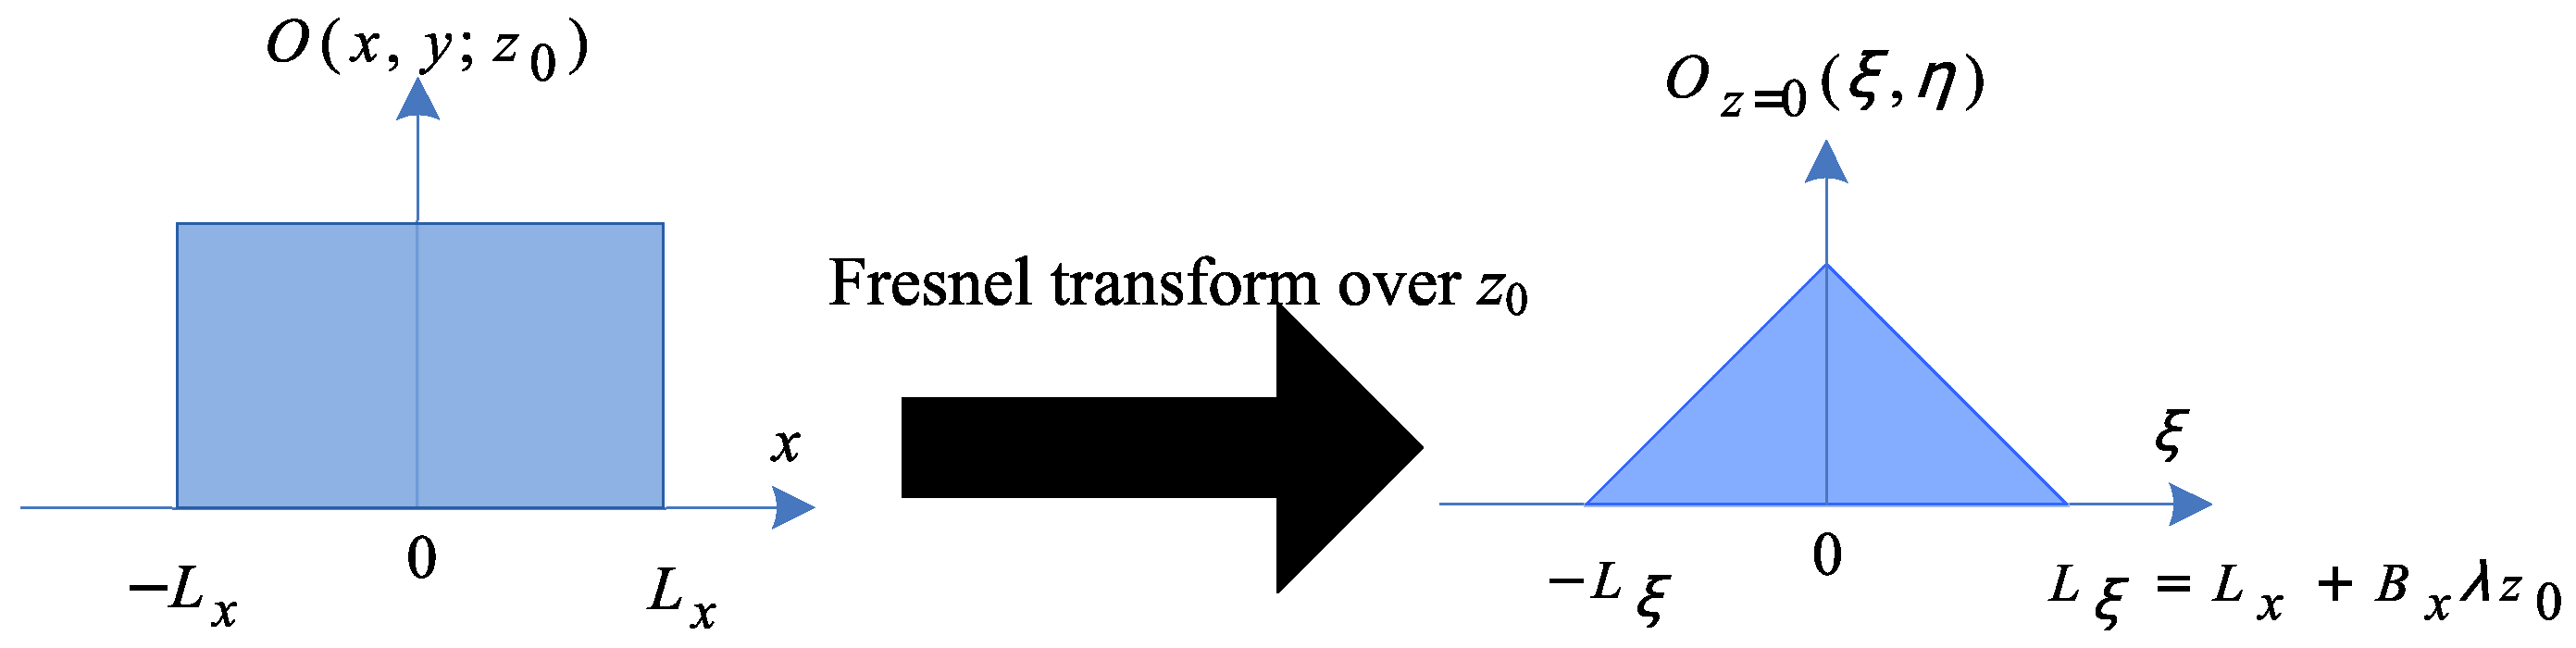
\includegraphics[width=.55\columnwidth]{fig_3}
\caption{Space domain representation of the object field at $z=z_0$ and $z=0$ plane.}
\label{fig_3}
\end{figure}

In the reconstruction, the object optical field at $z=0$, $O'_{z=0}(\xi', \eta')$ is obtained by taking Fourier transform of the hologram $H(u,v)$. Since the hologram is discretized with $\Delta u$, by the sampling theory, the reconstruction of the object at $z=0$ plane exhibits repetition of the original field, as shown in Fig.~\ref{fig_4}~\ref{Goodman_2005}. The repetition period of the reconstructed objects at $z=0$ plane is given by $\lambda f/\Delta u=\lambda/2\Delta\theta$. 

\begin{figure}[htbp]
\centering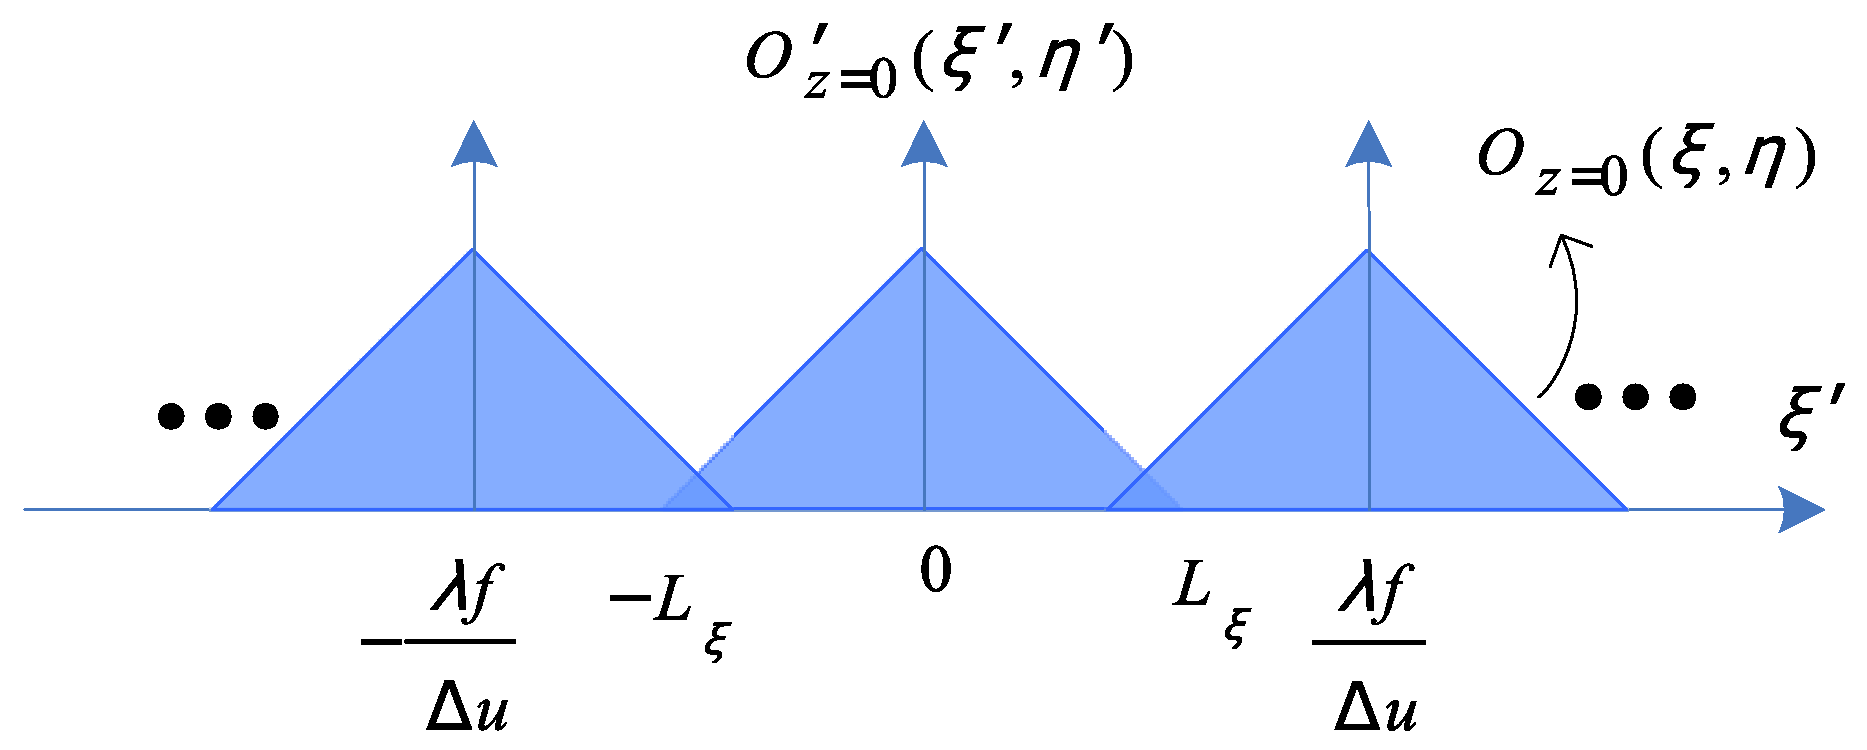
\includegraphics[width=.4\columnwidth]{fig_4}
\caption{Space domain representation of the reconstruction at $z=0$ plane.}
\label{fig_4}
\end{figure}

Figure~\ref{fig_5} is the final reconstruction at $z=z_0$ plane $O'(x', y'; z_0)$. This is obtained by taking Fresnel transform to $O_{z=0}'(\xi', \eta')$ over $z_0$. From Fig.~\ref{fig_5}, we can see that if we want to reconstruct the object without overlapping, we must satisfy inequality~(\ref{eq_6}). Following inequality~(\ref{eq_6}), the projection angle interval $\Delta\theta$ should be controlled to prevent overlapping of the reconstructed object.

\begin{equation}
\begin{aligned}
{L_x} \leqslant \frac{{\lambda f}}{{2\Delta u}} = \frac{\lambda }{{4\Delta \theta }}.
\end{aligned}
\label{eq_6}
\end{equation}

\begin{figure}[htbp]
\centering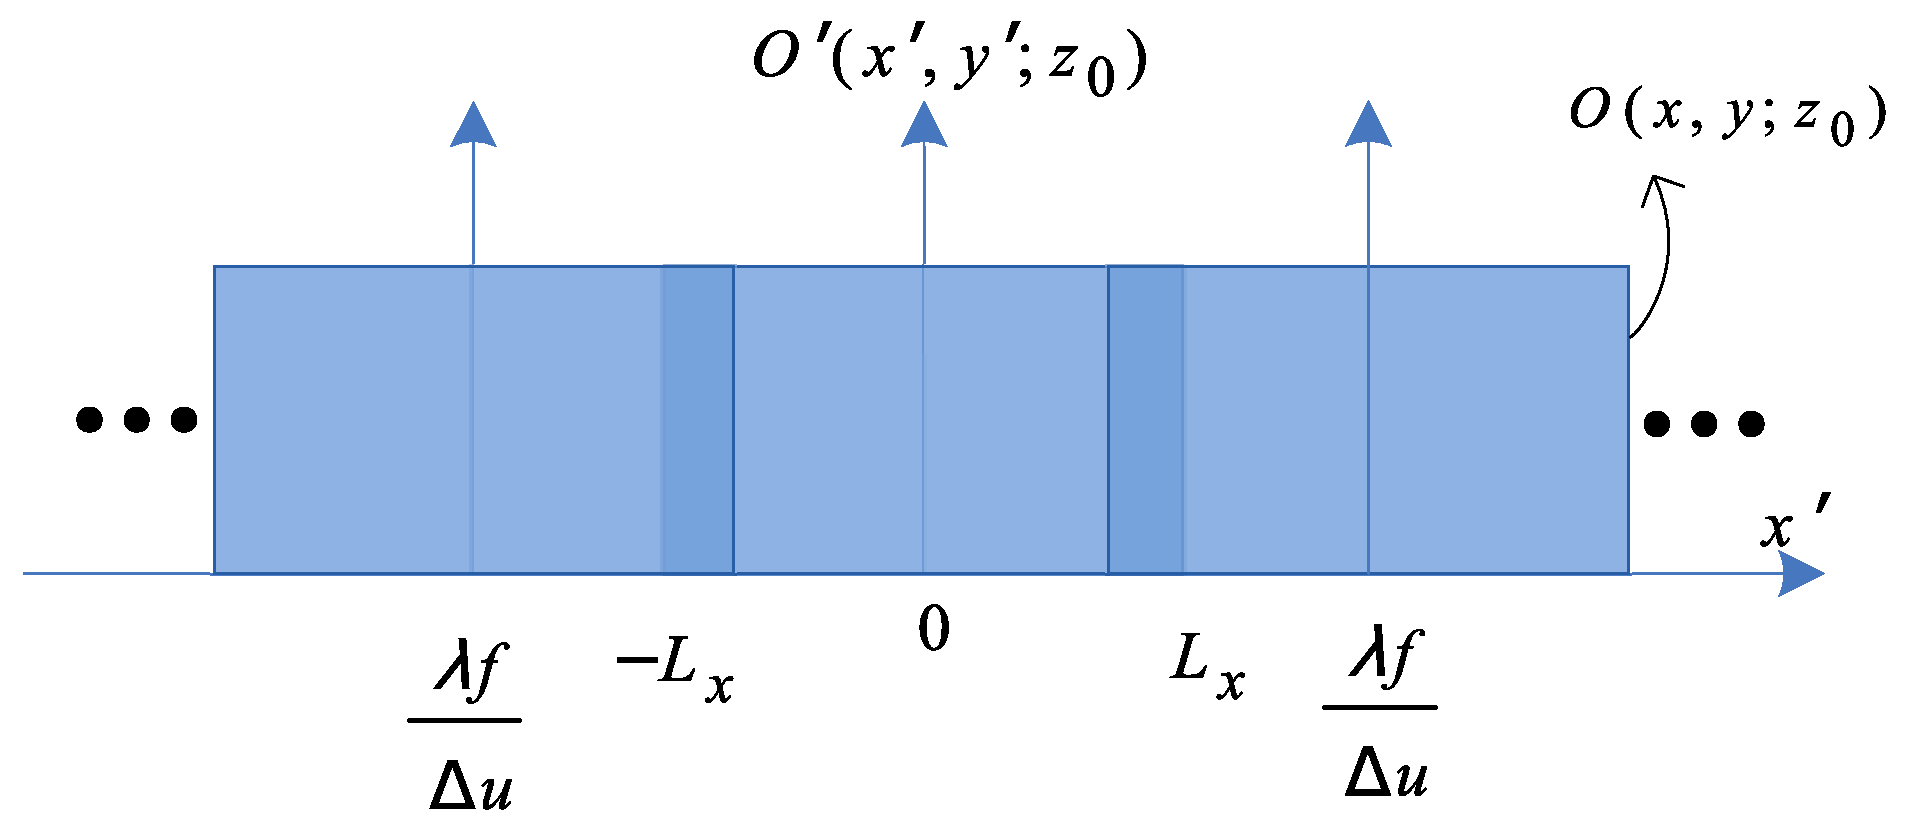
\includegraphics[width=.4\columnwidth]{fig_5}
\caption{Space domain representation of the reconstructed object at $z=z_0$.}
\label{fig_5}
\end{figure}

\subsection{Spatial frequency of the reconstructed object}
Figure~\ref{fig_6} shows the spatial frequency domain representation of the object at $z=z_0$ and $z=0$ plane. The bandwidth of the object is maintained after Fresnel propagation over distance $z_0$~\cite{Stern_2004_JOSA,Stern_2006_JOSA}.

\begin{figure}[htbp]
\centering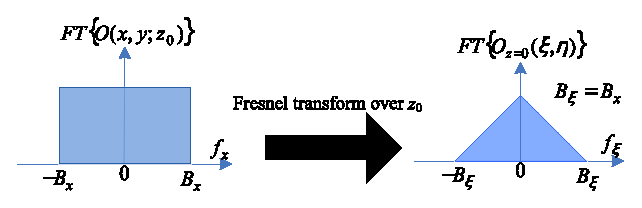
\includegraphics[width=.5\columnwidth]{fig_6}
\caption{Schematic of generation and reconstruction of the integral Fourier hologram.}
\label{fig_6}
\end{figure}

The main factors determining the resolution of the reconstruction are element lens pitch $\Delta x_p$ and the maximum projection angle $\theta_{max}$. In the integral Fourier hologram generation process, orthographic view images that are synthesized by collecting the pixels from every element image are used. Since only one pixel is extracted from each element image, the spatial sampling interval of the orthographic view image is given by the element lens pitch $\Delta x_p$. The 3D object is first sampled with $\Delta x_p$ in the orthographic view synthesis, and the orthographic view images are used in the hologram generation. Hence the reconstruction of the hologram reflects this sampling effect as a repetition of the original object field with $1/\Delta x_p$ period in the spatial frequency domain. Another factor that determines the reconstruction resolution is the maximum projection angle $\theta_{max}$. As discussed in previous section 2.1, the half size of the hologram Lu is determined by the maximum projection angle $\theta_{max}$ as $L_u=2 f\theta_{max}$. According to the sampling theorem, the maximum frequency of the reconstructed object from the Fourier hologram is given by~\cite{Goodman},
\begin{equation}
\begin{aligned}
{f_{x',\max }} = {f_{\xi ',\max }} = \frac{{{L_u}}}{{\lambda f}} = \frac{{2{\theta _{\max }}}}{\lambda },
\end{aligned}
\label{eq_7}
\end{equation}

\begin{figure}[htbp]
\centering
\includegraphics[width=.4\columnwidth]{fig_7}
\caption{Spatial frequency domain representation of the reconstruction at $z=0$ plane.}
\label{fig_7}
\end{figure}

\begin{equation}
\begin{aligned}
{B_x} = {B_\xi } \leqslant \frac{1}{{2\Delta {x_p}}}.
\end{aligned}
\label{eq_8}
\end{equation}

\begin{figure}[htb]
\centering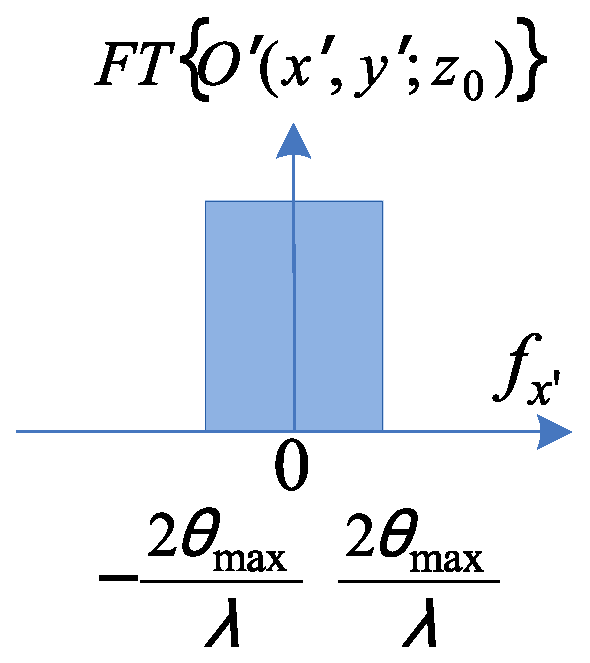
\includegraphics[width=.2\columnwidth]{fig_8}
\caption{Spatial frequency domain representation of the final reconstruction at $z=z_0$ plane.}
\label{fig_8}
\end{figure}

Figure~\ref{fig_8} is the reconstruction of the object at $z=z_0$. The maximum frequency is limited by the maximum projection angle in the element image capturing process and the wavelength. If we want to reconstruct the object without high frequency loss, assuming that there is no aliasing, the cutoff frequency $2\theta_{max}/\lambda$ given by Eq.~(\ref{eq_7}) must be larger than the bandwidth of the object,
\begin{equation}
\begin{aligned}
{B_x} < \frac{{2{\theta _{\max }}}}{\lambda }.
\end{aligned}
\label{eq_9}
\end{equation}
If there is aliasing, however, we need to make the cutoff frequency as large as possible while rejecting the aliased frequency region. The condition is given by
\begin{equation}
\begin{aligned}
\frac{2\theta _{\max}}{\lambda } < \frac{1}{\Delta x_p} - B_x.
\end{aligned}
\label{eq_10}
\end{equation}

\subsection{Principle of resolution enhanced Fourier hologram by using lens array shift method}
We have seen that there are several limitations in the Fourier hologram generation from multiple orthographic images. One is the limitation of the projection angle, which is one of the main factors that affect the maximum frequency of the reconstructed object from the hologram. The other factor is the sampling rate of the 3D objects, which is determined by the element lens pitch of the lens array. Large element lens pitch limits the bandwidth of the reconstruction according to Eq.~(\ref{eq_10}). In practical cases, the element lens pitch $\Delta x_p$ is not small enough to capture a 3D object of large bandwidth, making it the dominant factor limiting the resolution. It is possible to use a lens array with smaller lens pitch in order to increase the sampling rate. However, the lens pitch can not be reduced arbitrarily. In addition, a small lens pitch decreases the element image size, making it hard to capture an image with sufficient pixel count. It also decreases the maximum projection angle unless the f-number is maintained.
\begin{figure}[htbp]
\centering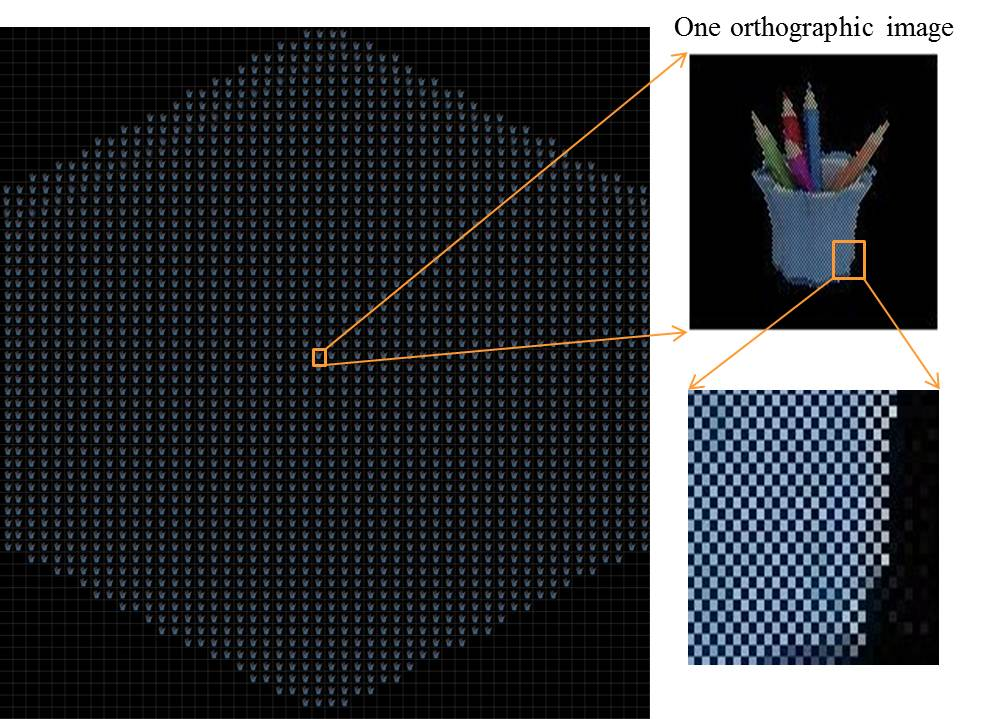
\includegraphics[width=.55\columnwidth]{fig_9}
\caption{Principle of lens array shift method. (a) Lens array shift in the vertical direction. (b) Synthesis of new set of the element images.}
\label{fig_9}
\end{figure}

The lens array shift method is one solution to this problem. We can use a lens array with proper lens pitch to maintain the maximum projection angle and sufficient element image pixel count, while increasing the sampling rate of the 3D object. In the lens array shift method, we capture four sets of element images and then combine the four sets of element images into one set of element images that has higher spatial density. Figure~\ref{fig_9}(a) shows the element images capturing process of the lens array shift method in the vertical direction. First, we set the lens array to a reference position and capture a set of element images. After this, the lens array is shifted along the vertical direction by half of the element lens pitch. With this lens array position, the other set of element images is captured. Then we shift the lens array along the horizontal direction over half of the lens pitch to the original reference lens array position and repeat the process to obtain another two sets of element images. Figure~\ref{fig_9}(b) shows the synthesis method using the four sets of element images. Four sets of element images are marked as $\text{EI}_{ij}$, where $i$ is the index in the horizontal direction and $j$ is the index in the vertical direction. The element images in each set of element images with the same index are gathered together as a group in the synthesized element image. The grouped four element images are located in the synthesized set according to their indexes as shown in Fig.~\ref{fig_9}(b). In the synthesized element images, the number of the element images is doubled, making the effective lens array pitch half. From this synthesized element images, integral Fourier hologram of higher resolution can be obtained.

\section{Simulation and experiment results}

\subsection{Verification of the parameter analysis}
We verified the parameter analysis computationally. Figure 10 is the object used in the simulation. The pixel count of the object is $200(H)\times200(V)$, the size is $0.1m(H)\times0.1m(V)$, and the bandwidth is $2B_x=2000$. The wavelength we used in the computational Fourier hologram generation and reconstruction is $500μm$. The distance of the object from the lens array is $0.2m$.
\begin{figure}[htbp]
\centering
\includegraphics[width=.25\columnwidth]{fig_10}
\caption{The object used in simulation}
\label{fig_10}
\end{figure}

\begin{table}[htbp]
\centering\caption{Simulation parameters to verify the overlapping theorem}
\begin{tabular}{l l l}
\hline
case  & $\Delta\theta$  & $\lambda/4\Delta \theta$     \\ \hline
I     & $0.1432^\circ$  & $10.003cm$                   \\ 
II    & $0.18^\circ$    & $7.9577cm$                   \\ \hline
\end{tabular}
\label{lb_1}
\end{table}

Table~\ref{lb_1} shows the parameters of the simulation to verify the maximum object size. According to all the other parameters and the previous analysis, the maximum $\Delta\theta$ that ensures no overlapping in the reconstructed object is $0.1432^\circ$. If $\Delta\theta$ is larger than this value, overlapping is expected to happen. Figure~\ref{fig_11} is the space domain representation of the reconstructed object with the parameters in Table 1. Figure~\ref{fig_11}(a) is the representation of case (I) and Fig.~\ref{fig_11}(b) is the representation of case (II).

\begin{figure}[htbp]
\centering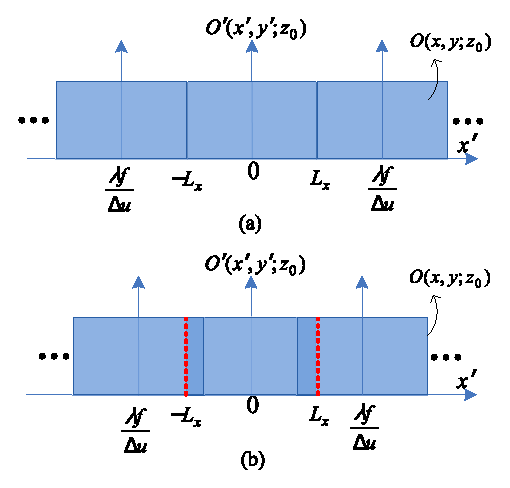
\includegraphics[width=.4\columnwidth]{fig_11}
\caption{Space domain representation of the reconstructed objects with the parameters in Table 1. (a) Case (I), (b) case (II). }
\label{fig_11}
\end{figure}

Figure~\ref{fig_12}(a) is the reconstruction with the parameters of case (I) in Table~\ref{lb_1}. The maximum allowable object size is nearly the same as the original object, thus there is no overlapping. Figure~\ref{fig_12}(b) is the reconstruction with the parameters of case (II) in Table 1. The $\Delta\theta$ is larger than the maximum $\Delta\theta$. With this $\Delta\theta$ the maximum allowable object size is $7.9577cm$, which is smaller than the original object size. In Fig.~\ref{fig_12}(b), as we expected, overlapping happens in the reconstruction. 
\begin{figure}[htbp]
  \centering
  \captionsetup[subfigure]{justification=centering}
  \begin{subfigure}[b]{0.22\linewidth}
  \centering
  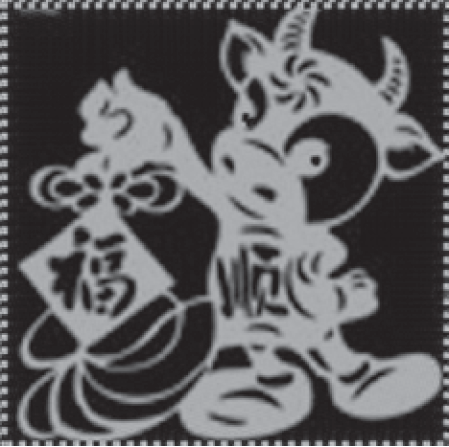
\includegraphics[width=1\columnwidth]{cow_overlapping_0}
  \caption{}
  \end{subfigure}
  \begin{subfigure}[b]{0.22\linewidth}
  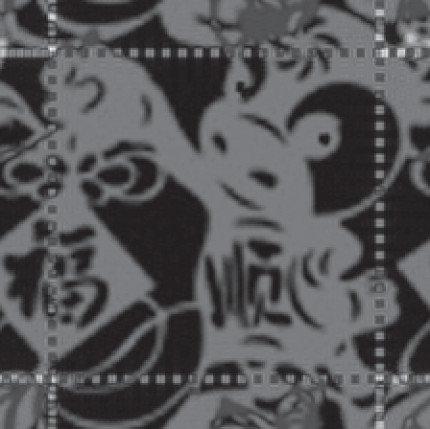
\includegraphics[width=1\columnwidth]{cow_overlapping_1}
  \centering
  \caption{}
  \end{subfigure}
\caption{Reconstructed images from the integral Fourier holograms using parameters in Table 1. (a) Case (I), (b) Case (II).}
\label{fig_12}
\end{figure}

\begin{table}[!htb]
\centering\caption{Simulation parameters to verify the overlapping theorem}
\begin{tabular}{l l l l}
\hline
case & $\theta_{max}$ & $2\theta_{max}/\lambda$ & $\Delta x_p$ \\ \hline
I    & $14.324°$      & 1000.0038               & 0.5mm        \\ 
II   & $14.324°$      & 1000.0038               & 0.91mm       \\ 
III  & $6°$           & 418.879                 & 0.5mm        \\ 
IV   & $6°$           & 418.879                 & 0.91mm       \\ \hline
\end{tabular}
\label{lb_2}
\end{table}

Table~\ref{lb_2} shows the simulation parameters to verify the maximum spatial frequency in the reconstruction. In cases (I) and (II), we verify the aliasing in the reconstruction, and case (III) and (IV) are used to verify the cutoff frequency. Here we maintained the small $\Delta\theta$ to reconstruct the object without any overlapping. From inequality (8), the maximum $\Delta x_p$ that avoids aliasing in the reconstruction is 0.5mm. If $\Delta x_p$ is larger than this value, there will be aliasing in the reconstruction. If the aliasing is very severe, the reconstruction will look like a collection of points. From inequality (9), the maximum projection angle $\theta_{max}$ that is required to avoid high frequency loss is $14.324^\circ$. In cases (III) and (IV), the $\theta_{max}$ is set to be smaller, so the cutoff frequency is smaller than the bandwidth of the object. In case (III), $\Delta x_p$ was set small to avoid the aliasing under the cutoff frequency. In case (IV), $\Delta x_p$ was increased to incur the aliasing under the cutoff frequency. Figures~\ref{fig_13}(a)-(d) are the spatial frequency domain representations of the reconstructions at $z=0$ plane of each case in Table~\ref{lb_2}.

\begin{figure}[htbp]
\centering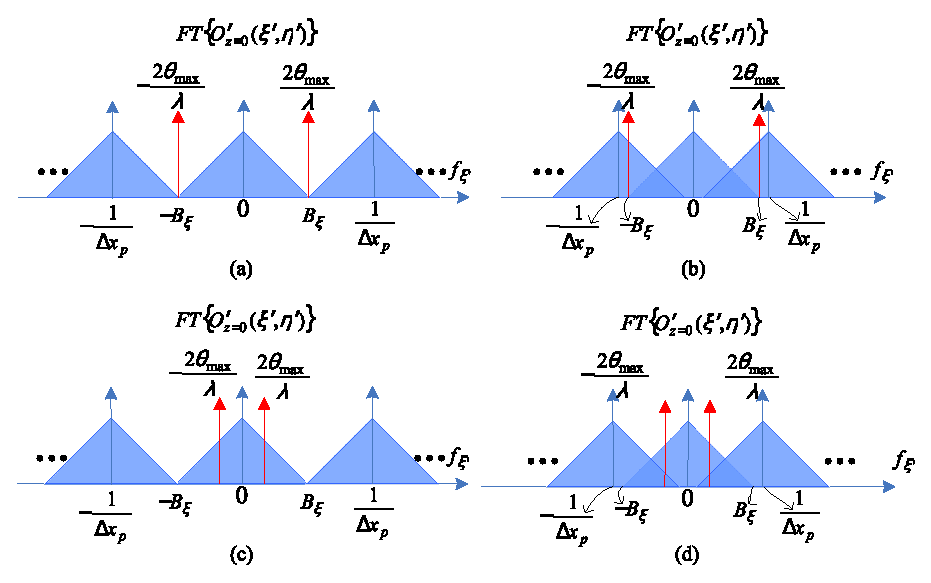
\includegraphics[width=.7\columnwidth]{fig_13}
\caption{Spatial frequency domain representation of the reconstructions at z=0 plane with the parameters in Table 2. (a)~Case(I), (b)~case (II). (c)~case (III), (d)~case (IV).}
\label{fig_13}
\end{figure}

% \begin{figure}[htbp]
% \centering\includegraphics[width=.55\columnwidth]{fig_14}
% \caption{Reconstructed images from the integral Fourier holograms using parameters in Table 1. (a) Case (I), (b) Case (II).}
% \label{fig_14}
% \end{figure}
\begin{figure}[htbp]
  \centering
  \captionsetup[subfigure]{justification=centering}
  \begin{subfigure}[b]{0.24\linewidth}
  \centering
  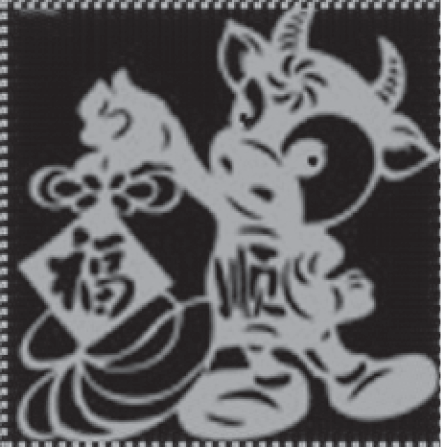
\includegraphics[width=1\columnwidth]{14-a}
  \caption{}
  \end{subfigure}
  \begin{subfigure}[b]{0.24\linewidth}
  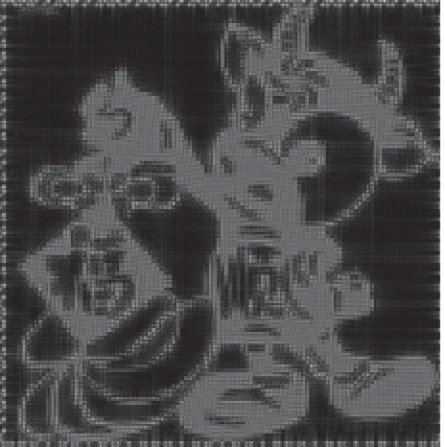
\includegraphics[width=1\columnwidth]{14-b}
  \centering
  \caption{}
  \end{subfigure}

 \begin{subfigure}[b]{0.24\linewidth}
  \centering
  
\includegraphics[width=1\columnwidth]{14-c}
  \caption{}
  \end{subfigure}
  \begin{subfigure}[b]{0.24\linewidth}
  
\includegraphics[width=1\columnwidth]{14-d}
  \centering
  \caption{}
  \end{subfigure}
\caption{Reconstructed images from the integral Fourier holograms using parameters in Table 1. (a) Case (I), (b) Case (II).}
\label{fig_14}
\end{figure}



The results are shown in Fig.~\ref{fig_14}. We can see that the resolution of Fig.~\ref{fig_14}(a) is the best because there is no aliasing and no frequency information loss. In Fig.~\ref{fig_14}(b), the aliasing makes the reconstructed image look like a collection of points. In Fig. ~\ref{fig_14}(c), the high frequency component of the object is lost; hence the details of the object at the edges are degraded. In Fig.~\ref{fig_14}(d), the aliasing happens, and also the high frequency information is lost; thus the image quality is deteriorated.

\subsection{Verification of the lens array shift method}
We verified the resolution enhancement of the integral Fourier hologram by using the lens array shift method experimentally. We performed two experiments, one with two plane objects and the other one with a real 3D object.

In the experiment, the objects were captured by a lens array. The lens array consists of identical elemental lenses of $1mm×1mm$ lens pitch and $3.3mm$ focal length. In the capturing process, we captured four sets of element images. We used a Sony DSLR $\alpha$900 to capture the element images. We first captured one set of element images, and then shifted the lens array horizontally $0.5mm$ and captured the second set of element images. To the third and fourth sets of element images, the lens array was shifted vertically $0.5mm$. We combined these four sets of element images into one set of element images with the proposed synthesis method as explained in section 2. Now we can regard this synthesized element images as one set of element images captured through a lens array with effective lens pitch of $0.5mm$. From the original single set of element images and this synthesized set of the element images, the orthographic images were generated separately~\cite{Park_2008_OE}; then, the Fourier Holograms were generated from the orthographic images. Finally the objects were reconstructed at different depths from these two integral Fourier holograms. 

In the experiment, the mechanical movement of the lens array may cause position errors in the lens array shift. Since the object is sampled at each elemental lens position in the orthographic image capture process, the position error of the lens array shift leads to non-uniform sampling of the object, i.e. the effective sampling interval is not a constant $\Delta x_p/2 $but fluctuates, which degrades final reconstruction quality by acting as broadband noise. 

In our experiment, the minimum unit of the translate stage was $0.01 mm$, which limits the maximum error of the lens array shifting under $0.01mm$. This maximum error $0.01mm$ corresponds to sub-pixel shift, or $0.5$ pixel shift, in terms of the captured elemental image pixel with our experimental setup (i.e. $\Delta x_p=1mm$, pixel count of each element image =$50$). Consequently, the error caused by the mechanical movement of the lens array could be ignored in our experiment.
\begin{figure}[!htb]
\centering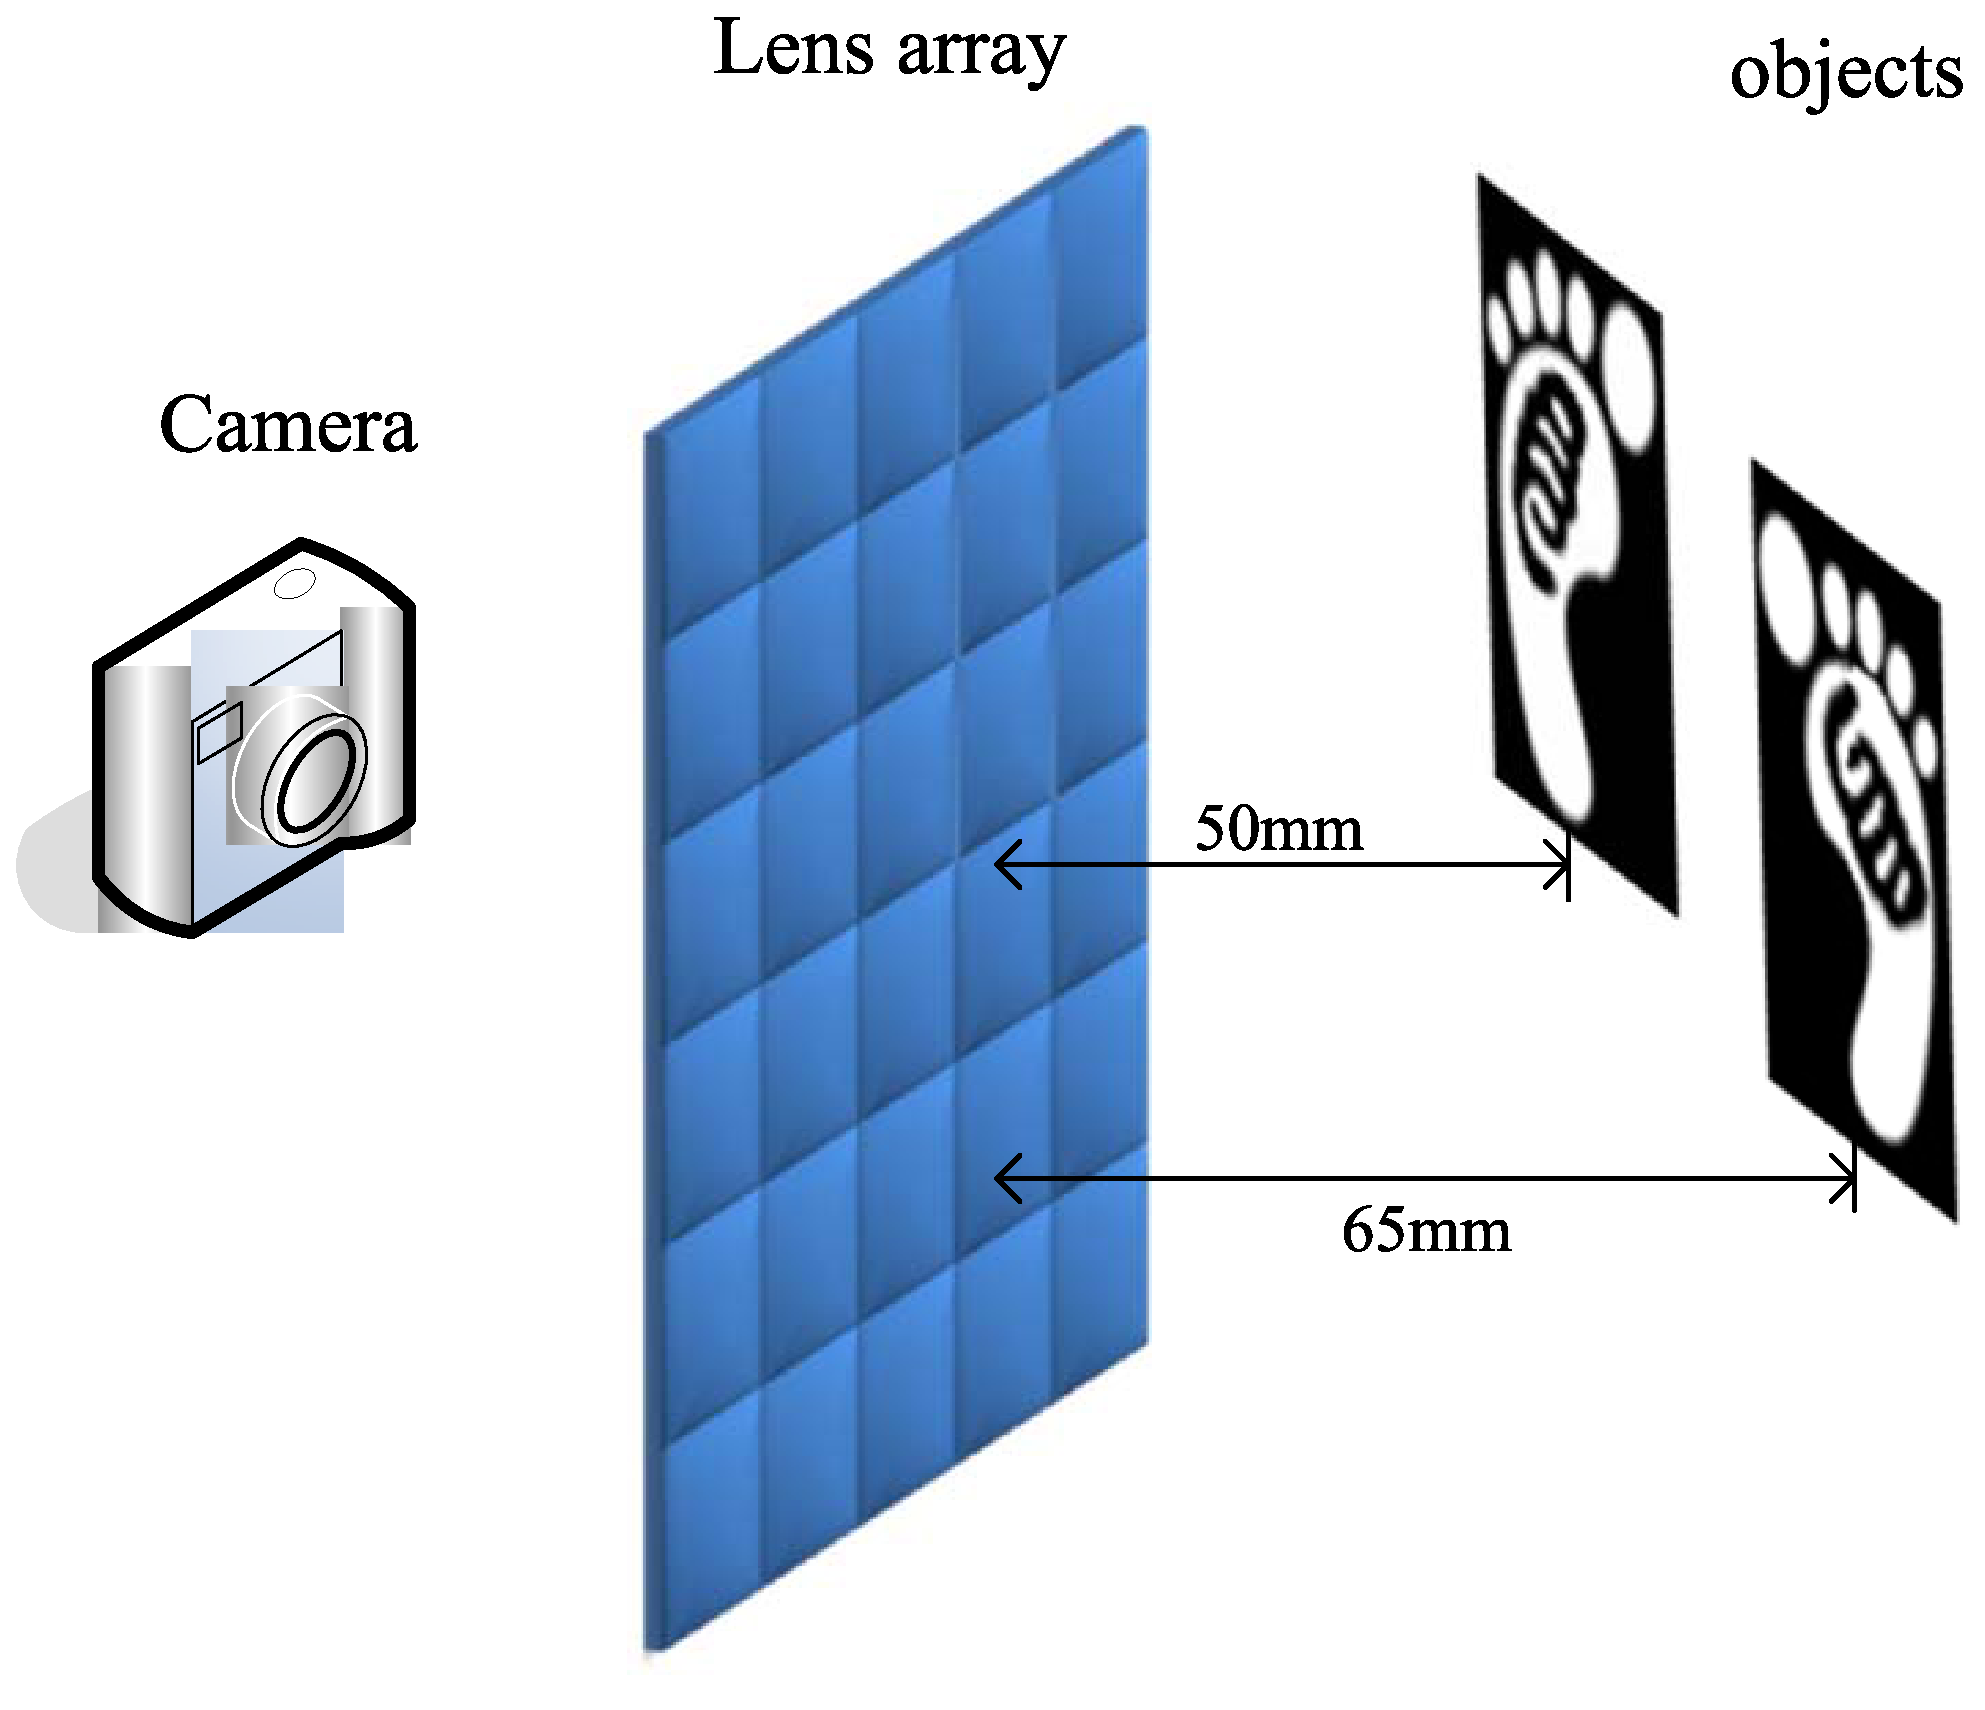
\includegraphics[width=.4\columnwidth]{fig_15}
\caption{Experimental setup to capture the element images of two plane objects}
\label{fig_15}
\end{figure}

In the two plane objects experiment, the objects were located away from the lens array at $50mm$ for the left footprint and $65mm$ for the right one. Figure 15 shows the experiment setup. The total lateral size of the two objects was $5.8(H) \times7.5(V)cm$. The pixel count of each element image was $50(H) \times50(V)$ pixels. Hence the pixel size of the element image $\Delta s$ was calculated to be 1mm/50=20μm and the angular separation between the projection lines was $\Delta\theta=20μm/3.3mm=0.3472^\circ$. In the computational reconstruction, the wavelength was set to $300μm$. With this $\Delta\theta$, the maximum allowable object size is $2.475cm$, which is much smaller than the real object size. Here we repeated each orthographic view image four times, making the effective $\Delta\theta$ be $\Delta\theta=0.3472^\circ/4=0.0868^\circ$. Since in our experiment the apparent differences between neighboring orthographic view images were negligible, this simple repetition can be justified. In general, the intermediate view reconstruction~(IVR) method can be used~\cite{Park_2008_OE,Zhang_2006_CSVT}. With reduced $\Delta\theta=0.0868^\circ$, the maximum allowable object size is now $9.9c$m, which is larger than the object we used. Thus we can reconstruct the object without overlapping.
\begin{figure}[!htb]
\centering
  \captionsetup[subfigure]{justification=centering}
  \centering\begin{subfigure}[b]{0.48\linewidth}
      \begin{tikzpicture}[scale=1, transform shape, font=\Large]
      \scope[nodes={inner sep=0,outer sep=0}]
        \node[anchor=south west] 
        {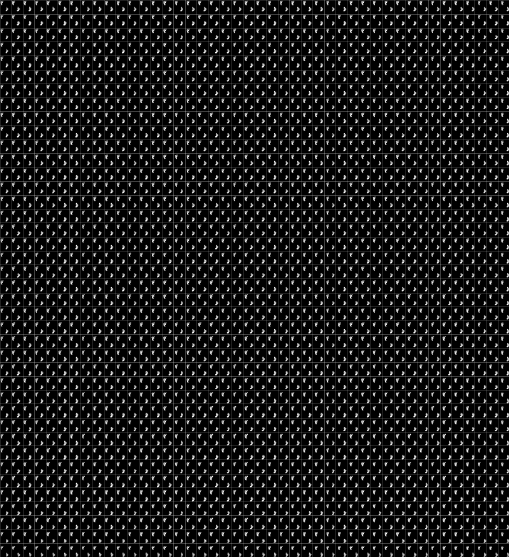
\includegraphics[width=1\linewidth]{foot_ei_conv} };
              \draw[yellow, thick] (3.2,3.5) rectangle (3.35,3.65);     
              \draw[thick,->,yellow] (3.2,3.5) -- (2.5, 0) node[anchor=north west] {};
              \draw[thick,->,yellow] (3.35,3.5) -- (4.05, 0) node[anchor=north west] {};
      \endscope
      \end{tikzpicture}

       \centering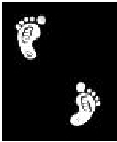
\includegraphics[width=0.3\linewidth]{foot_ei_conv1} 
  \caption{}
  \end{subfigure}
  \begin{subfigure}[b]{0.48\linewidth}
      \begin{tikzpicture}[scale=0.952, transform shape, font=\Large]
      \scope[nodes={inner sep=0,outer sep=0}]
        \node[anchor=south west] 
        {
\includegraphics[width=1\linewidth]{foot_ei_shift} };
              \draw[yellow, thick] (3.2,3.5) rectangle (3.35,3.65);          
              \draw[thick,->,yellow] (3.2,3.5) -- (2.5,0) node[anchor=north west] {};
              \draw[thick,->,yellow] (3.35,3.5) -- (4.05, 0) node[anchor=north west] {};
      \endscope
      \end{tikzpicture}

      \centering 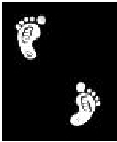
\includegraphics[width=0.3\linewidth]{foot_ei_conv1} 
  \caption{}
  \end{subfigure}
  % \begin{subfigure}[b]{1\linewidth}
  % 
\includegraphics[width=0.48\columnwidth]{foot_ei_shift}
  % \centering
  % \caption{}
  % \end{subfigure}
\caption{Element images and generated orthographic images. (a)~Conventional single set of element images (left figure) and orthographic images (right figure) generated from single set of element images. (b) Element images (left figure) synthesized from 4 sets of the elemental images captured with lens array shifting and orthographic images (right figure) generated from synthesized element images.}
\label{fig_16}
\end{figure}

 % \centering
 %  \begin{subfigure}[b]{1\linewidth}
 %      \centering\begin{tikzpicture}[scale=0.6, transform shape, font=\Large]
 %      \scope[nodes={inner sep=0,outer sep=0}]
 %        \node[anchor=south west] 
 %        {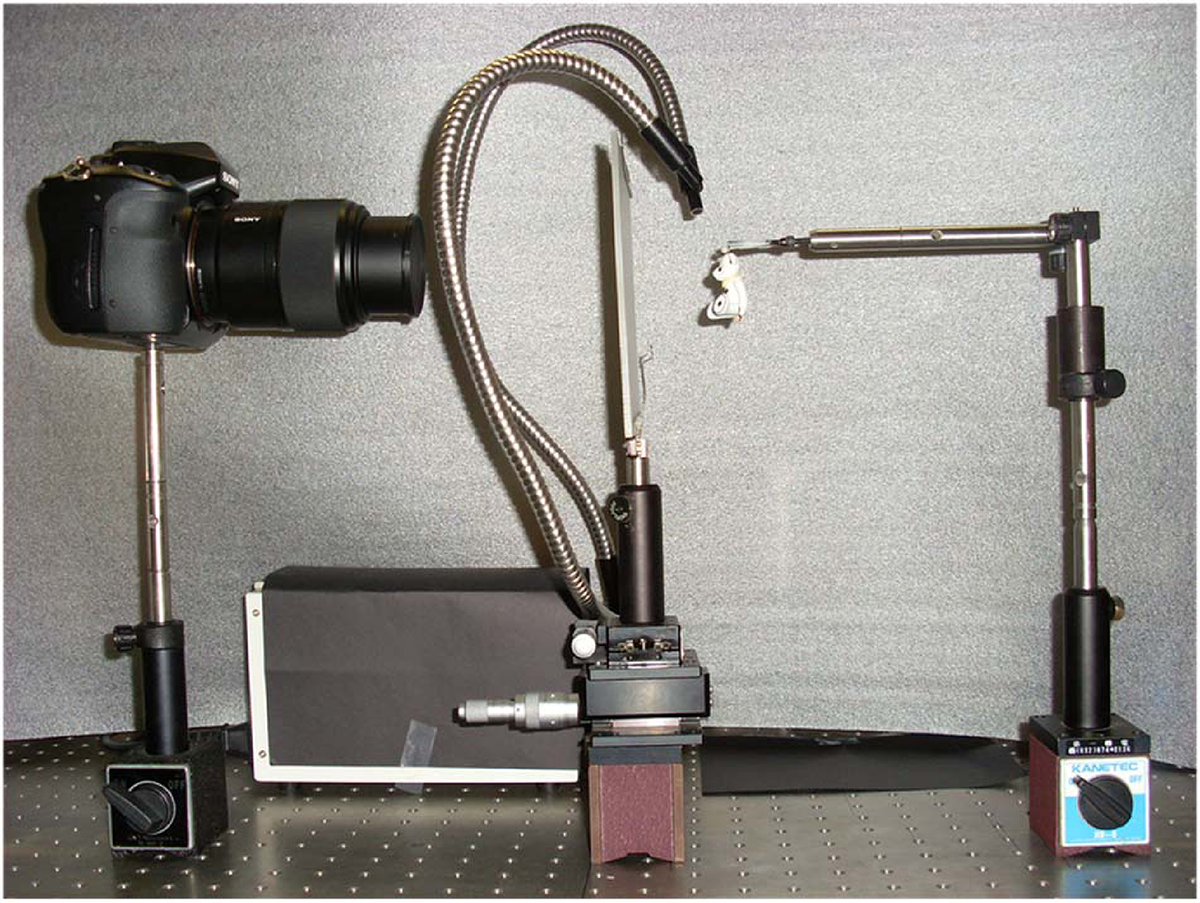
\includegraphics[width=1\linewidth]{fig_18a} };
 %             \draw (1.5,7) node {$\textcolor{yellow}{Camera}$};  
 %              \draw (8.8,8.7) node {$\textcolor{yellow}{Illumination}$};  
 %              \draw (9.2,6.8) node {$\textcolor{yellow}{Object}$};  

 %              \draw[yellow, thick] (5,1.5) rectangle (7.9,3.3);     
 %              \draw[thick,->,yellow] (6.5, 1.5) -- (6.8, 1.1) node[anchor=north west] {$\textcolor{yellow}{Translation Stage}$};

 %               \draw[yellow, thick] (6.5,4.7) rectangle (7.3,8.7);     
 %              \draw[thick,->,yellow] (7.3, 5.5) -- (7.9, 5) node[anchor=north west] {$\textcolor{yellow}{Lens array}$};
 %      \endscope
 %      \end{tikzpicture}
 %      \caption{}
 %   \end{subfigure}
    
 %    \begin{subfigure}[b]{0.7\linewidth}
 %        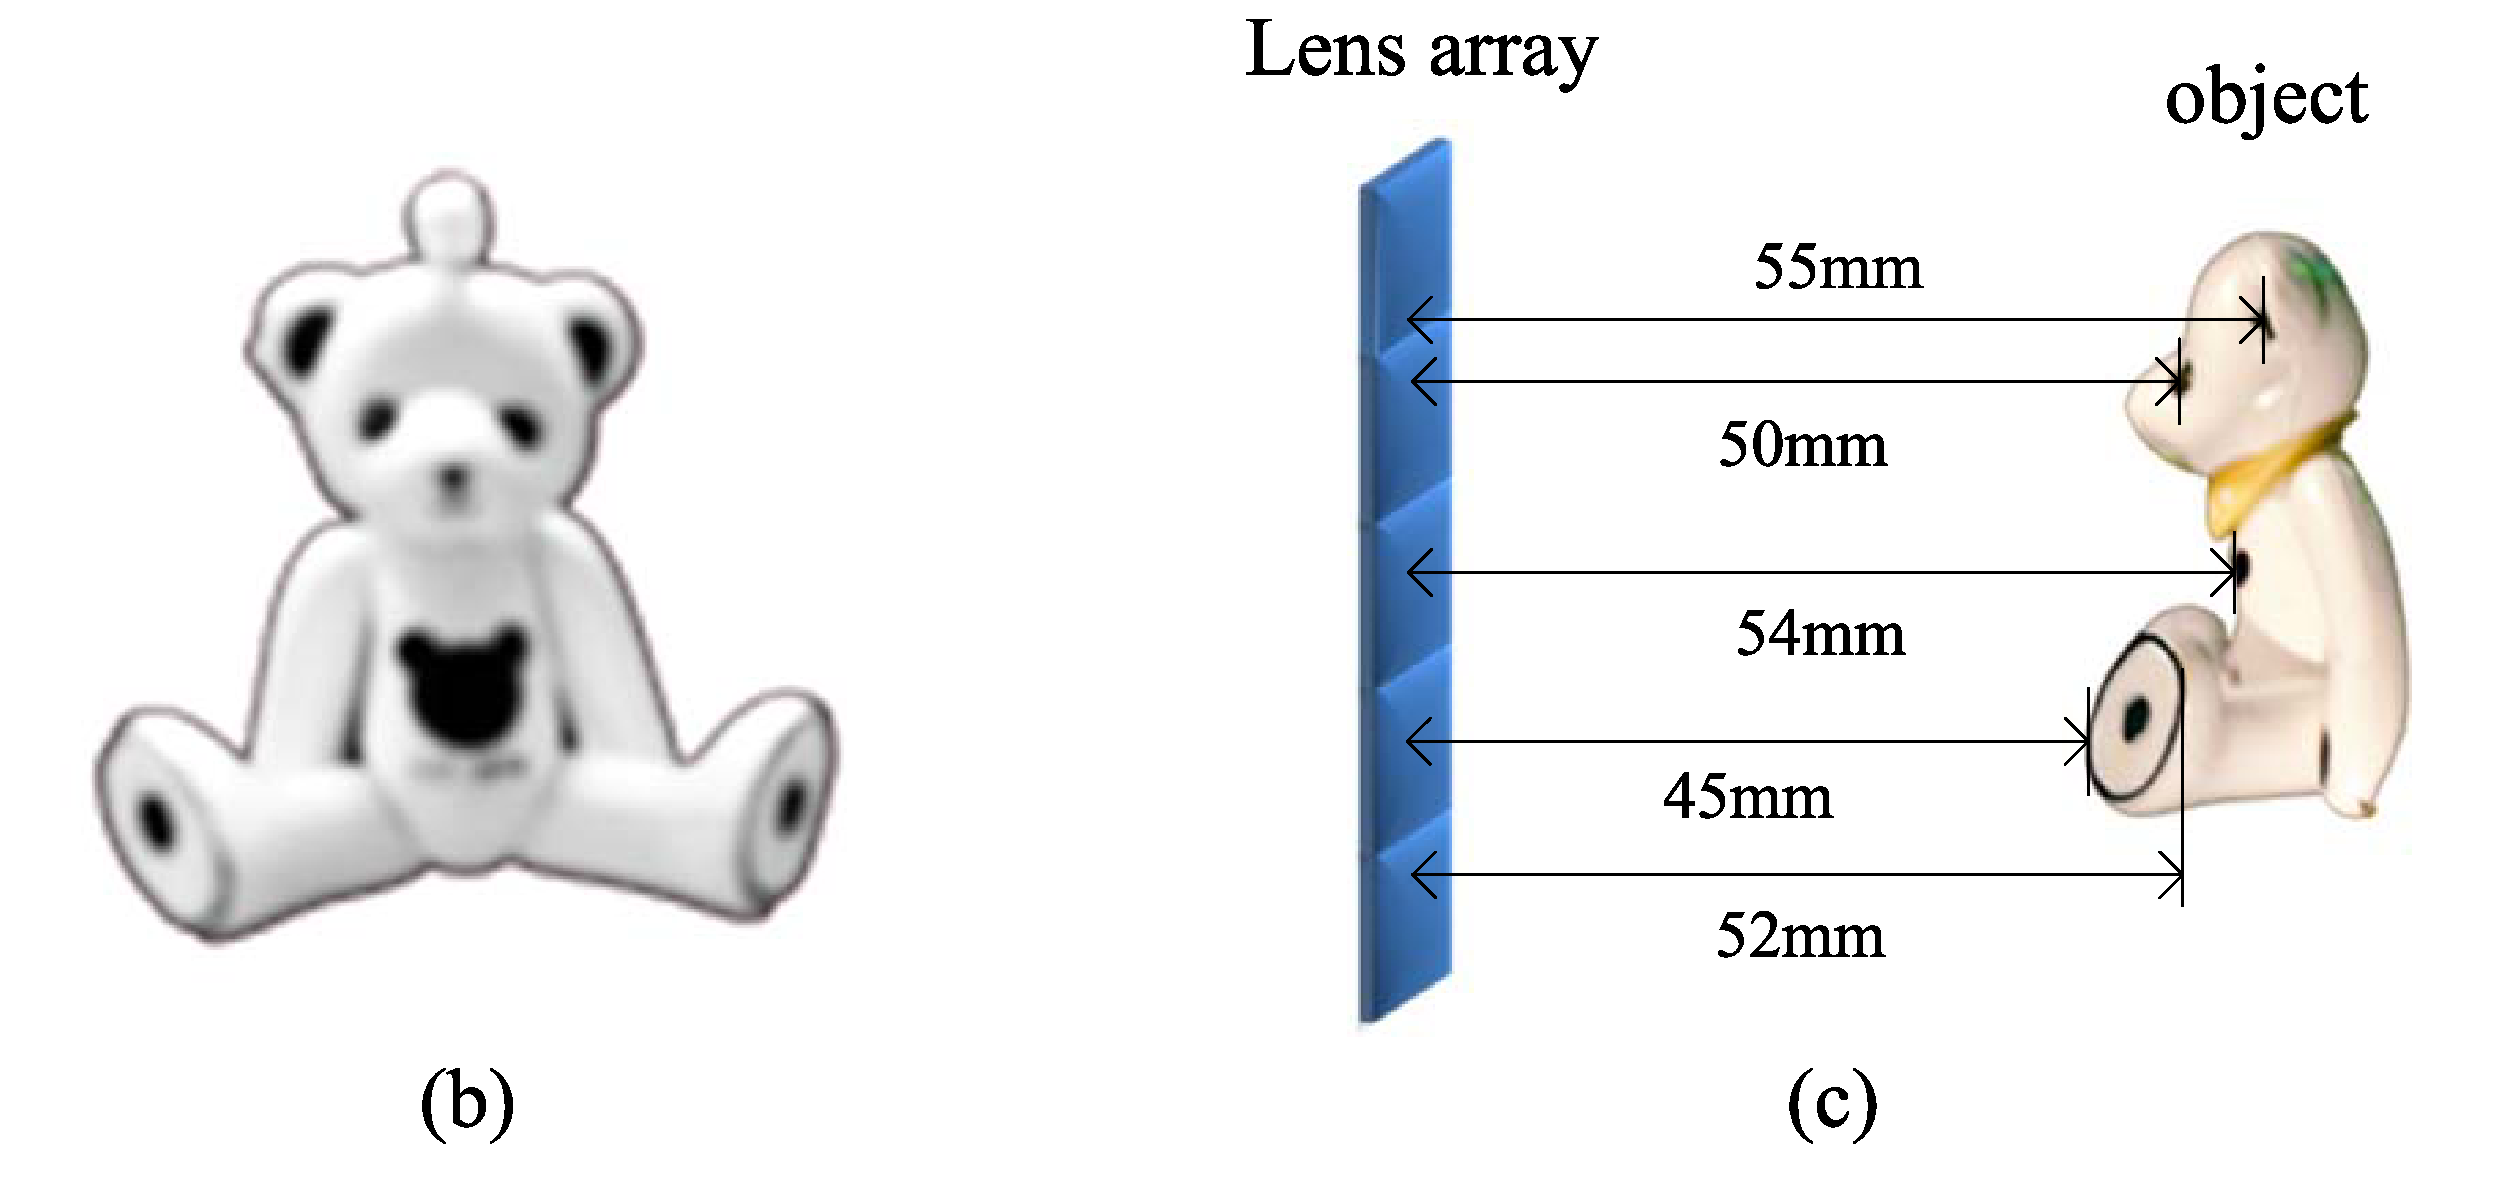
\includegraphics[width=1\linewidth]{fig_18b} 
 %        % \caption{}
 %   \end{subfigure}

Figure~\ref{fig_16}(a) shows the conventional element images and orthographic images and Fig.~\ref{fig_16}(b) is the element images and orthographic images taken using the lens array shift method. With the lens array shift method, the number of the element images is doubled. Hence pixel count of each orthographic image is doubled.

Figure~\ref{fig_17}(a) shows the conventional reconstructed objects with different depths. The left footprint is reconstructed at a distance of $50mm$ and the right footprint is reconstructed at $65mm$. The reconstructions are degraded because of the aliasing. Figure~\ref{fig_17}(b) is the reconstructed object done by using the lens array shift method. We can see that by using the lens array shift method, the resolution of the reconstruction is enhanced over the conventional one.
% \begin{figure}[htbp]
% \centering
% \includegraphics[width=.8\columnwidth]{fig_17}
% \caption{Reconstruction of two plane objects. (a) Reconstruction from conventional integral Fourier hologram generated from a single set of element images, (b) reconstruction from proposed integral Fourier hologram generated with lens array shift method.}
% \label{fig_17}
% \end{figure}

\begin{figure}[htbp]
\centering
  \vspace{2pt} 
   \begin{overpic}[width=.2\linewidth]{foot_0_35}
  \end{overpic}
  \begin{overpic}[width=.2\linewidth]{foot_0_50}
  \end{overpic}
    \begin{overpic}[width=.2\linewidth]{foot_0_65}
  \end{overpic}
    \begin{overpic}[width=.2\linewidth]{foot_0_80}
  \end{overpic}
   \centerline{(a)}

    \vspace{2pt} 
   \begin{overpic}[width=.2\linewidth]{foot_1_35}
  \end{overpic}
  \begin{overpic}[width=.2\linewidth]{foot_1_50}
  \end{overpic}
    \begin{overpic}[width=.2\linewidth]{foot_1_65}
  \end{overpic}
    \begin{overpic}[width=.2\linewidth]{foot_1_80}
  \end{overpic}
   \centerline{(b)}
\caption{Reconstruction of two plane objects. (a) Reconstruction from conventional integral Fourier hologram generated from a single set of element images, (b) reconstruction from proposed integral Fourier hologram generated with lens array shift method.}
\label{fig_17}
\end{figure}


\begin{figure}[!htb]
% \centering\includegraphics[width=.6\columnwidth]{fig_18}
 \centering
  \begin{subfigure}[b]{1\linewidth}
      \centering\begin{tikzpicture}[scale=0.6, transform shape, font=\Large]
      \scope[nodes={inner sep=0,outer sep=0}]
        \node[anchor=south west] 
        {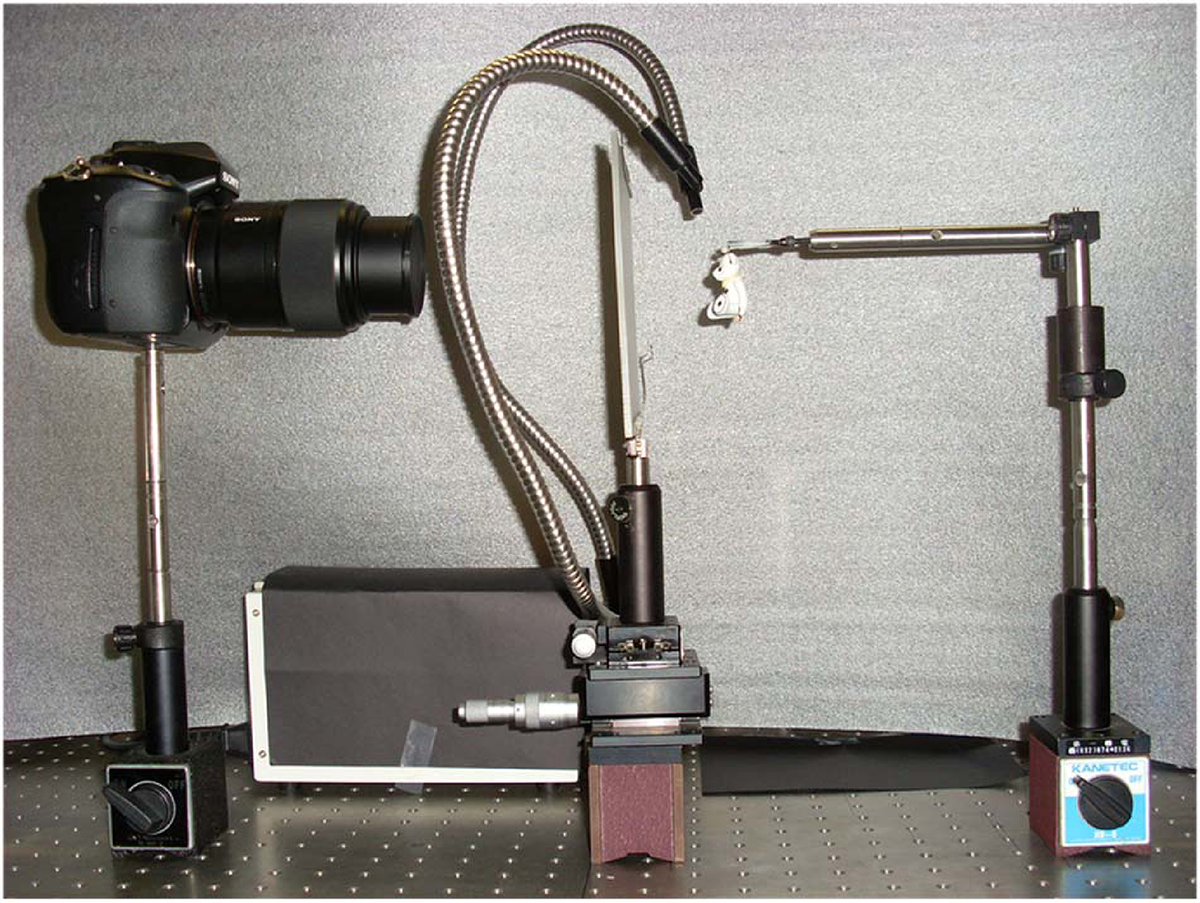
\includegraphics[width=1\linewidth]{fig_18a} };
             \draw (1.5,7) node {$\textcolor{yellow}{Camera}$};  
              \draw (8.8,8.7) node {$\textcolor{yellow}{Illumination}$};  
              \draw (9.2,6.8) node {$\textcolor{yellow}{Object}$};  

              \draw[yellow, thick] (5,1.5) rectangle (7.9,3.3);     
              \draw[thick,->,yellow] (6.5, 1.5) -- (6.8, 1.1) node[anchor=north west] {$\textcolor{yellow}{Translation Stage}$};

               \draw[yellow, thick] (6.5,4.7) rectangle (7.3,8.7);     
              \draw[thick,->,yellow] (7.3, 5.5) -- (7.9, 5) node[anchor=north west] {$\textcolor{yellow}{Lens array}$};
      \endscope
      \end{tikzpicture}
      \caption{}
   \end{subfigure}
    
    \begin{subfigure}[b]{0.7\linewidth}
        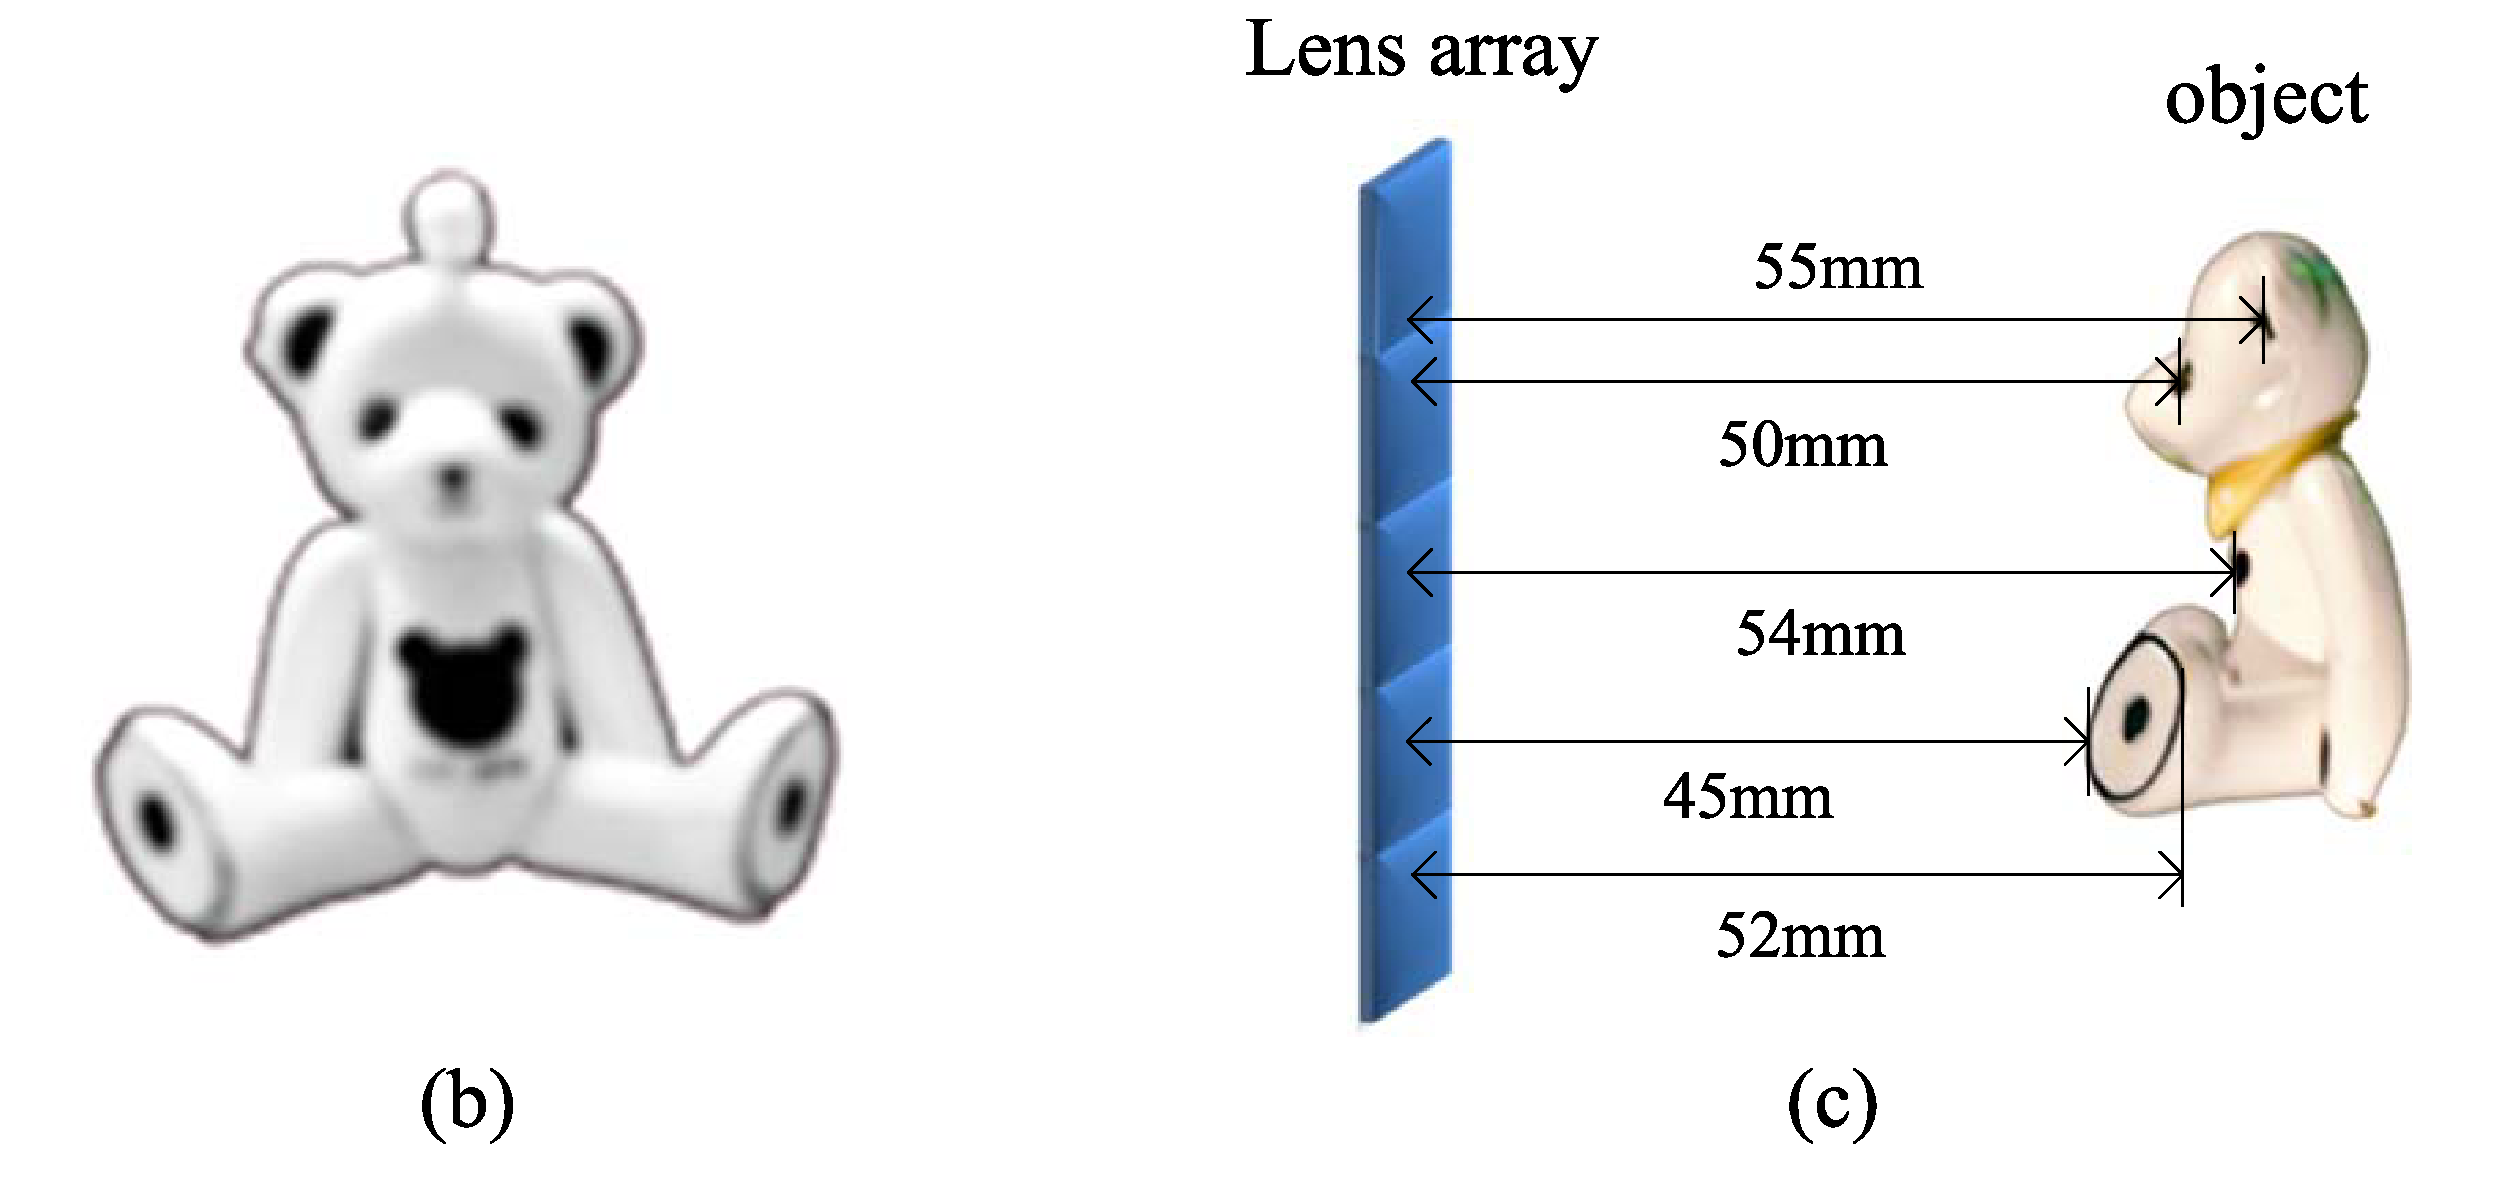
\includegraphics[width=1\linewidth]{fig_18b} 
        % \caption{}
   \end{subfigure}
\caption{Experimental setup to capture the element images. (a) The experimental setup to capture the real 3D object, (b) frontal image of the object. (c) the distances from the lens array to the different parts of the object.}
\label{fig_18}
\end{figure}

We also applied the proposed method to real 3D objects of continuous depth profile. Figure~\ref{fig_18}(a) is the experimental setup. All the experimental setup is the same as in the above experiment except for the object. Figure~\ref{fig_18}(b) is the two dimensional image of the real 3D object we used in the experiment. Figure~\ref{fig_18}(c) shows the distances to the lens array from different parts of the object. The size of the object is $4cm(H)\times4cm (V)$. In this experiment, the pixel count of the element image was $54(H)\times54(V)$; hence the pixel size of the element image was $1mm/54=18.52μm$. The angular separation between the projection lines was $\Delta\theta=18.52μm/3.3mm=0.3216^\circ$. In the reconstruction, the wavelength was 300μm. With this $\Delta\theta$, the maximum allowable object size is $2.673cm$. Hence we also doubled the number of the orthographic view images by repeating them twice~\cite{Park_2008_OE,Zhang_2006_CSVT}. $\Delta\theta$was decreased to $0.1608^\circ$, making the maximum allowable object size 5.346cm.
\begin{figure}[!htb]
\centering
    \vspace{2pt} 
   \begin{overpic}[width=.24\linewidth]{bear_holo_amp_conv}
  \end{overpic}
  \begin{overpic}[width=.24\linewidth]{bear_holo_phase_conv}
  \end{overpic}
   \centerline{(a)}

    \vspace{2pt} 
   \begin{overpic}[width=.24\linewidth]{bear_holo_amp_shift}
  \end{overpic}
  \begin{overpic}[width=.24\linewidth]{bear_holo_phase_shift}
  \end{overpic}
   \centerline{(b)}

\caption{Amplitude (left figures) and phase (right figures) of the generated Fourier hologram. (a) Conventional integral Fourier hologram. (b) Integral Fourier hologram by using Lens shift method.}
\label{fig_19}
\end{figure}

% \begin{figure}[htbp]
% \centering\includegraphics[width=.45\columnwidth]{fig_19}
% \caption{Amplitude (left figures) and phase (right figures) of the generated Fourier hologram. (a) Conventional integral Fourier hologram. (b) Integral Fourier hologram by using Lens shift method.}
% \label{fig_19}
% \end{figure}

\begin{figure}[!htb]
\centering
  \begin{overpic}[width=.12\linewidth]{bear_0_45}
  \put(-25,25){\rotatebox[origin=tl, units=360]{90}{(a)}}
  \put(1,105){\color{black}{$z=45mm$}}
  \end{overpic}
  \begin{overpic}[width=.12\linewidth]{bear_0_48}
  \put(1,105){\color{black}{$z=48mm$}}
  \end{overpic}
  \begin{overpic}[width=.12\linewidth]{bear_0_51}
  \put(1,105){\color{black}{$z=51mm$}}
  \end{overpic}
  \begin{overpic}[width=.12\linewidth]{bear_0_54}
   \put(1,105){\color{black}{$z=54mm$}}
  \end{overpic}
  \begin{overpic}[width=.12\linewidth]{bear_0_57}
   \put(1,105){\color{black}{$z=57mm$}}
  \end{overpic}
  \begin{overpic}[width=.12\linewidth]{bear_0_60}
   \put(1,105){\color{black}{$z=60mm$}}
  \end{overpic}
  \begin{overpic}[width=.12\linewidth]{bear_0_63}
   \put(1,105){\color{black}{$z=63mm$}}
  \end{overpic}

  \vspace{2pt} 
  \begin{overpic}[width=.12\linewidth]{bear_1_45}
  \put(-25,25){\rotatebox[origin=tl, units=360]{90}{(b)}}
  \end{overpic}
  \begin{overpic}[width=.12\linewidth]{bear_1_48}
  \end{overpic}
  \begin{overpic}[width=.12\linewidth]{bear_1_51}
  \end{overpic}
  \begin{overpic}[width=.12\linewidth]{bear_1_54}
  \end{overpic}
  \begin{overpic}[width=.12\linewidth]{bear_1_57}
  \end{overpic}
  \begin{overpic}[width=.12\linewidth]{bear_1_60}
  \end{overpic}
  \begin{overpic}[width=.12\linewidth]{bear_1_63}
  \end{overpic}

    \vspace{2pt} 
  % \begin{overpic}[width=.12\linewidth]{bear_1_45}
  % \put(-25,25){\rotatebox[origin=tl, units=360]{90}{(b)}}
  % \end{overpic}
   \begin{overpic}[width=.24\linewidth]{bear_0_48}
  \end{overpic}
  \begin{overpic}[width=.24\linewidth]{bear_1_48}
  \end{overpic}
   \centerline{(c)}


\caption{Reconstruction of the 3D object’s Fourier hologram. (a) Conventional integral Fourier hologram generated from a single set of element images (b) Proposed integral Fourier hologram generated using lens shift method, (c) Comparison of the reconstructions at $z=54mm$.}
\label{fig_20}
\end{figure}

% \begin{figure}[htbp]
% \centering\includegraphics[width=.8\columnwidth]{fig_20}
% \caption{Reconstruction of the 3D object’s Fourier hologram. (a) Conventional integral Fourier hologram generated from a single set of element images (b) Proposed integral Fourier hologram generated using lens shift method, (c) Comparison of the reconstructions at $z=54mm$.}
% \label{fig_20}
% \end{figure}

Figure~\ref{fig_19} shows the generated Fourier holograms. Figure~\ref{fig_19}(a) is the amplitude and phase of the conventional Fourier hologram, and Fig.~\ref{fig_19}(b) is the amplitude and phase of the Fourier hologram made using the lens array shift method. Figure~\ref{fig_20} shows the reconstruction from the Fourier holograms in Fig.~\ref{fig_19}. Figure~\ref{fig_20}(a) is the conventional reconstruction; the object reconstruction is degraded because of the aliasing. Figure~\ref{fig_20}(b) is the reconstruction from the Fourier hologram made using the lens array shift method. Figure~\ref{fig_20}(c) is the comparison of the magnified reconstruction at $z=54mm$ in Fig.~\ref{fig_process}(a) and Fig.~\ref{fig_process}(b).It can be confirmed that the resolution is enhanced by the lens array shift method. It is also clearly seen that different parts of the object are reconstructed correctly at different depths; the left foot at about $48mm$, the eyes at $51mm$, the picture in the belly at about $54mm$, and the legs clearly at about $63mm$. 

\section{Conclusion}
In this paper, we presented an analysis of the parameters that affect the resolution of the reconstruction of an integral Fourier hologram. It was found that the projection angle interval between neighboring orthographic view images determines the maximum size of the reconstruction field. It was also found that the maximum projection angle and the element lens pitch of the lens array determine the maximum spatial frequency of the reconstruction. Based on this analysis, the resolution enhancement using the lens array shifting method was proposed. The simulation and experimental results confirmed the validity of the analysis and the feasibility of the resolution enhancement by the lens array shift method. 

\section*{Acknowledgments} 
``This work was partly supported by a grant of the Korean Ministry of Education, Science and Technology" (The Regional Core Research Program/Chungbuk BIT Research-Oriented University Consortium)''\\

\noindent ``This research was partly supported by National Research Foundation of Korea Grant funded by the Korean Government(2009-0069677)''

\end{document}
